%
% A Universidade Estadual Paulista "Júlio de Mesquita Filho"            
% MODELO DE  RELATÓRIO 
%
\documentclass[
	% -- opções da classe memoir --
	12pt,				% tamanho da fonte
	openright,			% capítulos começam em pág ímpar (insere página vazia caso preciso)
	oneside,			% para impressão em verso e anverso. Oposto a oneside
	a4paper,			% tamanho do papel. 
	% -- opções da classe abntex2 --
	%chapter=TITLE,		% títulos de capítulos convertidos em letras maiúsculas
	%section=TITLE,		% títulos de seções convertidos em letras maiúsculas
	%subsection=TITLE,	% títulos de subseções convertidos em letras maiúsculas
	%subsubsection=TITLE,% títulos de subsubseções convertidos em letras maiúsculas
	% -- opções do pacote babel --
	english,			% idioma adicional para hifenização
	french,				% idioma adicional para hifenização
	spanish,			% idioma adicional para hifenização
	brazil				% o último idioma é o principal do documento
	]{abntex2}

%test

% Pacotes básicos 
\usepackage[alf]{abntex2cite}
\usepackage{chngcntr}
\counterwithout{footnote}{chapter}
\counterwithout{equation}{chapter}
\usepackage{lmodern}			% Usa a fonte Latin Modern			
\usepackage[T1]{fontenc}		% Selecao de codigos de fonte.
\usepackage[utf8]{inputenc}		% Codificacao do documento (conversão automática dos acentos)
\usepackage{lastpage}			% Usado pela Ficha catalográfica
\usepackage{indentfirst}		% Indenta o primeiro parágrafo de cada seção.
\usepackage{color}				% Controle das cores
\usepackage{graphicx}			% Inclusão de gráficos
\usepackage{microtype} 			% para melhorias de justificação
\usepackage{afterpage}
\usepackage{amsmath}
\usepackage{amssymb,url}
\usepackage{hhline}
\usepackage{xcolor,tikz,bm,colortbl}
\usepackage[ruled,linesnumbered,vlined,portuguese,onelanguage]{algorithm2e}

%Weslley-lars
\usepackage{float}
\usepackage{longtable,ltcaption} % para as tabelas
\usepackage{hyperref} %citacoes customizadas
\usepackage{rotating}
\usepackage{pdflscape}
\usepackage{longtable}
\usepackage{adjustbox}
\usepackage{adjustbox}
\usepackage{lipsum}
\usepackage{pdfpages}
\usepackage{longtable}
\usepackage{rotating} % para usar o ambiente 'sidewaystable'
%\usepackage{biblatex}
%\usepackage[style=numeric]{biblatex}  % Include the biblatex package




% -- Carregando o pacote do bloco de código: 
\usepackage{listings}
\lstset{
    literate={á}{{\'a}}1
           {ã}{{\~a}}1
           {ç}{{\c{c}}}1
           {í}{{\'i}}1
           {ú}{{\'u}}1,         
    language=Python,
    breaklines=true,
    basicstyle=\ttfamily\small,
    commentstyle=\color{olive},
    keywordstyle=\color{blue},
    numberstyle=\tiny\color{gray},
    numbers=left,
}
% -- Definindo cores: 
% -- Definindo um estilo personalizado: 



% Algumas mudanças devem ser realizadas neste arquivo, por exemplo, financiadora do projeto
\usepackage{0-libs/customizacoes}


% Informações de dados para CAPA e FOLHA DE ROSTO
\titulo{AIOPs - Utilizando uma Arquitetura Transformer em Time Series com Prometheus}
\autor{Weslley Rosalem}
\local{Bauru}
\data{2023}
\orientador{Prof. Dr. Kelton Augusto C. Pontara}
\instituicao{}
\tipotrabalho{Dissertação de Mestrado Acadêmico}
% O preambulo deve conter o tipo do trabalho, o objetivo, 
% o nome da instituição e a área de concentração 
\preambulo{Dissertação apresentada como parte dos requisitos para obtenção do título de Mestre em Ciência da Computação, junto ao Programa de Pós-Graduação em Ciência da Computação, do Instituto de Biociências, Letras e Ciências Exatas da Universidade Estadual Paulista “Júlio de Mesquita Filho", Câmpus de Bauru.}
% ---

% Configurações de aparência do PDF final

% alterando o aspecto da cor preta
\definecolor{black}{RGB}{0,0,0}
\definecolor{blue}{RGB}{0,0,190}

% informações do PDF
\makeatletter
\hypersetup{
     	%pagebackref=true,
		pdftitle={\@title}, 
		pdfauthor={\@author},
    	pdfsubject={\imprimirpreambulo},
	    pdfcreator={LaTeX com abnTeX2},
		pdfkeywords={abnt}{latex}{abntex}{abntex2}{dissertação}, 
		colorlinks=true,       		% false: boxed links; true: colored links
    	linkcolor=blue,          	% color of internal links
    	citecolor=blue,        		% color of links to bibliography
    	filecolor=magenta,      		% color of file links
		urlcolor=black,
		bookmarksdepth=4
}
\makeatother

% O tamanho do parágrafo é dado por:
\setlength{\parindent}{1.3cm}

% Controle do espaçamento entre um parágrafo e outro:
\setlength{\parskip}{0.2cm}  % tente também \onelineskip

% compila o indice
\makeindex
% ---

% ----
% Início do documento
% ----
\begin{document}

% Seleciona o idioma do documento (conforme pacotes do babel)
%\selectlanguage{english}
%\selectlanguage{brazil}


% Retira espaço extra obsoleto entre as frases.
\frenchspacing % ----------------------------------------------------------
% ELEMENTOS PRÉ-TEXTUAIS
% ----------------------------------------------------------
% Capa
\imprimircapa
% ---
% Folha de rosto
% (o * indica que haverá a ficha bibliográfica)
\imprimirfolhaderosto*

% Inserir Resumo e Abstract
%\chapter{Resumo}
%\label{cap:resumo}
\begin{resumo}

Com a crescente transformação digital, gerenciar ambientes de TI que são ao mesmo tempo complexos e dinâmicos, tornou-se um desafio cada vez maior. A inteligência Artificial em Operações de TI ou (AIOps), surge como uma solução que integra aprendizado de máquina e \textit{big data} para automatizar tarefas de gerenciamento de TI, tais como detecção de anomalias, previsão de capacidade, correlação de eventos e identificação de causas raízes. O objetivo principal deste estudo é combinar a arquitetura \textit{Transformer}, com dados de séries temporais provenientes do \textit{Prometheus}, sistema de monitoramento e banco de dados de séries temporais, a fim de melhorar a análise preditiva e a detecção de anomalias em sistemas de TI. A pesquisa realiza uma revisão sistemática da literatura, fundamentando as bases teóricas das tecnologias discutidas. A seção metodológica detalha os conjuntos de dados utilizados, as etapas de pré-processamento e as técnicas de análise preditiva adotadas. Os resultados deste estudo podem contribuir significativamente para a eficiência das operações de TI, facilitando o gerenciamento das complexidades presentes nos ambientes atuais.

\textbf{Palavras-chave:} \textit{Deep Learning; Time Series; Transformer; AIOPs}.

\end{resumo}

\begin{resumo}[\textit{Abstract}]
\textit{With the increasing digital transformation, managing IT environments, which are both complex and dynamic, has become an ever-greater challenge. Artificial Intelligence in IT Operations, or AIOps, emerges as a solution integrating machine learning and big data to automate IT management tasks, such as anomaly detection, capacity forecasting, event correlation, and root cause identification. The primary goal of this study is to combine the Transformer architecture with time series data from Prometheus, a monitoring system and time series database, to enhance predictive analysis and anomaly detection in IT systems. The research conducts a systematic review of the literature, establishing the theoretical foundations of the discussed technologies. The methodological section details the data sets used, the preprocessing steps, and the adopted predictive analysis techniques. The results of this study can significantly contribute to the efficiency of IT operations, facilitating the management of complexities present in current environments.}


\textbf{Keywords:} \textit{Deep Learning; Time Series; Transformer; AIOPs}.
\end{resumo}

% ---

% ---
% inserir lista de ilustrações
% ---
\pdfbookmark[0]{\listfigurename}{lof}
\listoffigures*
\cleardoublepage
% ---

% ---
% inserir lista de tabelas
% ---
\pdfbookmark[0]{\listtablename}{lot}
\listoftables*
\cleardoublepage
% ---

% inserir lista de abreviaturas e siglas
% ---
\begin{siglas}
\item [AI] - \textit{Artificial Intelligence}
\item[AIOPs] - \textit{Artificial Intelligence for IT Operations}
\item[CAM] - \textit{Class Activation Mapping }
\item [CNN] - \textit{Convolutional Neural Network}
\item[CVAE] - \textit{Conditional Variational Autoencoder}
\item[CPU] - \textit{Central Processing Unit}
\item[DevOps] - Desenvolvimento e Operações de TI
\item[DP] - \textit{Deep Learning}
\item[GRU] - \textit{Gated Recurrent Unit}
\item[HAC] - \textit{Hierarchical Agglomerative Clustering}
\item[IT] - \textit{Information Techonology}
\item[K8s] - \textit{Kubernetes}
\item[LSTM] - \textit{Long short-term memory}
\item [MAE] - \textit{Mean Absolute Error}
\item[ML] - \textit{Machine Learning}
\item[MLOPs] - \textit{Machine Learning Operations}
\item [NLP] - \textit{Natural Language Processing}
\item[NNET] - \textit{Neural Network}
\item[KPI] - \textit{Key Performance Indicator}
\item[RMSE] - \textit{Root Mean Squared Error}
\item[RNN] - \textit{Recurrent neural network}
\item[TF] - \textit{Transformer}
\item[TS] - \textit{Time Series}
\item [TI] - Tecnologias da informação
\item [TIC] - Tecnologias da informação e comunicação
\item[TSTF] - \textit{Time Series Transformer}


\end{siglas}
% ---


% inserir o sumario
\pdfbookmark[0]{\contentsname}{toc}
\tableofcontents
\cleardoublepage

% ----------------------------------------------------------
% ELEMENTOS TEXTUAIS
% ----------------------------------------------------------
\pagestyle{simple}

% ----------------------------------------------------------

%\input{chapters/2-ex1}
%\input{chapters/3-ex2}
%\input{chapters/4-ex3}
%\input{chapters/5-conclusao}
\chapter{INTRODUÇÃO} \label{cap_introducao}

Em meio à era da transformação digital, os ambientes de Tecnologia da Informação (TI), evoluíram para atender diversos cenários críticos, de diferentes setores, incluindo mas não limitando-se a: saúde, financeiro, telecomunicações, segurança, logística, entre outros. Visando melhorar a disponibilidade, resiliência,  flexibilidade e confiabilidade, eles também tornaram-se notavelmente mais complexos e dinâmicos. A crescente dependência das empresas em infraestruturas de TI para conduzir suas operações diárias, tem impulsionado a implementação de sistemas distribuídos em larga escala que são intrinsecamente desafiadores de monitorar, escalar, manter e prever a quantidade de recursos necessários \cite{pahl2015containerization}.

O gerenciamento desses vastos ambientes de TI é desafiador, dada a sua natureza heterogênea e a multiplicidade de componentes de hardware e software que integram. Os ambientes de TI contemporâneos englobam uma variedade de sistemas, desde servidores físicos, máquinas virtuais, contêineres, redes, bancos de dados e aplicações \cite{pahl2015containerization}. A adoção crescente da computação em nuvem amplia ainda mais essa complexidade, com recursos de TI distribuídos geograficamente.

Nesse cenário, as operações de TI são pressionadas a garantir a disponibilidade e o ótimo desempenho  desses sistemas. Uma das tarefas mais árduas é a identificação de causa raiz, que busca determinar a origem de falhas ou problemas em um sistema. Esta tarefa é exacerbada pela interdependência dos componentes e pela vastidão de dados gerados \cite{cohen2004correlating}.

A manutenção por sua vez, apresenta seus próprios desafios. Assegurar sistemas atualizados e protegidos contra vulnerabilidades, demanda monitoramento contínuo e frequentemente, a coordenação de atualizações em múltiplos sistemas. O processo de manutenção precisa ser meticuloso para minimizar interrupções em serviços  críticos.

Diante desses desafios, as organizações buscam soluções que possam automatizar e otimizar suas operações. A Inteligência Artificial para Operações de TI, conhecida como \textit{Artificial Inteligence for I.T Operations} (AIOps), emerge como uma disciplina que emprega técnicas de IA para abordar problemas operacionais. AIOps integra \textit{big data}\footnote{\textit{Big Data} refere-se a conjuntos de dados que são tão grandes e complexos que exigem métodos avançados e ferramentas de análise para processar. Estes dados podem ser estruturados ou não estruturados e são caracterizados por volume, velocidade e variedade.}
 e aprendizado de máquina, visando aprimorar aspectos como detecção de anomalias, previsão de capacidade, correlação de eventos e identificação de causas raízes \cite{sill2019aiops}.

No âmbito do AIOps, destaca-se o uso de aprendizado profundo\footnote{Aprendizado profundo, ou \textit{deep learning}, é uma subárea da aprendizagem de máquina \textit{(machine learning)}, que por sua vez é um domínio da inteligência artificial (IA). Essa técnica se inspira na estrutura e funcionamento do cérebro humano, mais especificamente nas redes neurais biológicas, para processar dados e criar padrões para a tomada de decisões.} para análise de séries temporais\footnote{Uma série temporal é uma sequência de pontos de dados coletados ou registrados em intervalos de tempo regulares ou irregulares. Cada ponto de dados na série temporal é um registro de alguma atividade, observação ou medição em um momento específico. Tecnicamente, uma série temporal é uma sequência de observações  x(t), onde  (t) representa o tempo em que a observação foi feita.}, como métricas de desempenho (KPI). A arquitetura \textit{Transformer}, originalmente concebida para processamento de linguagem natural, tem se mostrado eficaz em modelar complexidades em séries temporais, capturando dependências de longo alcance \cite{vaswani2017attention}.

Ademais, o \textit{Prometheus}, um sistema de monitoramento e banco de dados de séries temporais, é amplamente adotado para coletar métricas de sistemas de TI. Ao integrar arquitetura \textit{Transformer} com métricas do \textit{Prometheus}, é possível desenvolver modelos de aprendizado de máquina mais robustos para análise preditiva e detecção de anomalias.

Neste trabalho, será explorado a aplicação de \textit{Transformer} em dados de séries temporais obtidos via \textit{Prometheus}, visando identificar anomalias e prever tendências de consumo de recursos. Esta abordagem tem o potencial de aprimorar substancialmente a eficiência das operações de TI, facilitando o gerenciamento da crescente complexidade dos ambientes atuais. Nos capítulos subsequentes, serão abordados os fundamentos teóricos das tecnologias em foco, a metodologia adotada e os resultados alcançados, bem como a estrutura organizacional da pesquisa, sendo:

\begin{itemize}
    \item (Capítulo \ref{cap_introducao}), em que é apresentado o tema objeto da pesquisa de forma com que sejam justificados os esforços na realização da presente dissertação, bem como realizada a contextualização, apresentados os objetivos geral e específicos e a metodologia empregada;
    \item (Capítulo \ref{cap_fundamentacao-teorica} ), onde é mostrado o estado atual através de uma Revisão Sistemática da Literatura. Mostra ao leitor uma linha do tempo sobre a evolução do tema pesquisado nos últimos cinco anos.
    \item (Seção \ref{sec-arquitetura-transformer}), em que é documentada a arquitetura \textit{Transformer}, explorando seu mecanismo de atenção, codificador e decodificador, e outros componentes relevantes nesta arquitetura.
    \item (Seção \ref{cap-anal-pre-trans-ts}), onde é abordada a aplicação da arquitetura proposta com foco em \textit{forecast} para um conjunto de dados que contém métricas de um servidor real, armazenadas e coletadas em formato de série temporal.
    \item (Capítulo \ref{Cap_metodologia}), é documentado toda metodologia, detalhes do conjunto de dados, estratégia de pré-processamento e métricas utilizadas para avaliação da arquitetura.
    \item  (Capítulo \ref{Cap_resultados-preliminares}), neste capítulo são abordados os resultados parciais obtidos até o presente momento, contextualização e objetivos, e a configuração experimental.
    \item (Capítulo \ref{Cap_conclusao}), é apresentada a conclusão parcial, cronograma contendo as atividades a serem realizadas até a defesa desta dissertação, como a publicação de artigos relacionados ao tema, além da evolução do modelo e documentação dos resultados obtidos. 
\end{itemize}

A problemática que pautou o desenvolvimento desta Dissertação de Mestrado foi: uma arquitetura de \textit{deep learning} baseada em \textit{transformers}, aplicada à análise de métricas de dispositivos de ambientes de TI, pode contribuir de maneira proativa para a melhoria da eficiência operacional e resiliência?

Esta pesquisa é justificada pela crescente complexidade dos sistemas de TI e pelo aumento volumétrico de dados gerados, desafiando as práticas operacionais tradicionais. Atualmente, muitas operações de TI ainda são executadas manualmente e adotam uma abordagem reativa, o que pode ser inadequado diante da criticidade e da dinâmica dos sistemas modernos. A automação e a proatividade, facilitadas pelo uso de \textit{machine learning}, são essenciais para a gestão eficiente desses ambientes. A análise de séries temporais, em particular, oferece um meio robusto para a detecção precoce de anomalias e a previsão de tendências, contribuindo para a prevenção de falhas e a otimização de recursos. Portanto, esta dissertação contribui para o campo acadêmico ao explorar a aplicabilidade de técnicas avançadas de aprendizado de máquina em um contexto operacional crítico, fornecendo \textit{insights} valiosos para a evolução das práticas de AIOps.
\chapter{Fundamentação Teórica}
\label{cap_fundamentacao-teorica}

Este capítulo aborda os conceitos e teorias fundamentais que embasam este estudo. A compreensão desses conceitos é essencial para entender as técnicas e metodologias adotadas ao longo deste trabalho. Inicialmente, é discutida a evolução da Inteligência Artificial (IA). Em seguida, é focado no subcampo da IA denominado \textit{AIOps} (Inteligência Artificial para Operações de TI), que integra IA e análise de dados visando aprimorar as operações de TI. A familiaridade com IA e AIOps é vital para perceber como essas tecnologias podem ser aplicadas em ambientes de TI, potencializando a detecção de anomalias e a análise preditiva de séries temporais.

\section{Revisão Sistemática da Literatura}
\label{cap_revisao-sistematica}

A Revisão Sistemática da Literatura é uma abordagem metodológica que busca identificar, avaliar e interpretar todas as pesquisas relevantes sobre um tema específico. Distingue-se por sua metodologia rigorosa e bem definida, que pode ser replicada e auditada, conferindo maior confiabilidade ao processo utilizado \cite{tranfield2003systematic}.

Essa metodologia é empregada para coletar e sintetizar evidências empíricas que atendam a critérios de inclusão pré-estabelecidos \cite{kitchenham2007guidelines}. O processo envolve a definição de questões de pesquisa pertinentes, a seleção e avaliação qualitativa dos estudos, a extração de dados, a síntese e apresentação da documentação dos achados.

\subsection{Técnicas para Revisão Sistemática da Literatura}
\label{subcap_tec_rev-sistematica}

A Revisão Sistemática é fundamental na pesquisa acadêmica, pois oferece uma visão holística do conhecimento existente, destacando lacunas que podem ser objeto de futuras investigações \cite{petticrew2006systematic}. Além disso, evita a duplicação de esforços, evidenciando pesquisas prévias sobre o tema.

A elaboração de uma revisão sistemática é iniciada com a definição de um protocolo rígido de pesquisa. Neste protocolo, são estabelecidos critérios de inclusão e exclusão, as bases de dados a serem consultadas e as estratégias de busca a serem adotadas \cite{biolchini2005systematic}. A figura \ref{fig:processo_rev_sistematica} apresenta uma ilustração mais detalhes sobre procedimento adotado neste estudo:

\begin{figure}[H]
    \centering
    \caption{Procedimento adotado para realização da Revisão Sistemática da Literatura.}
    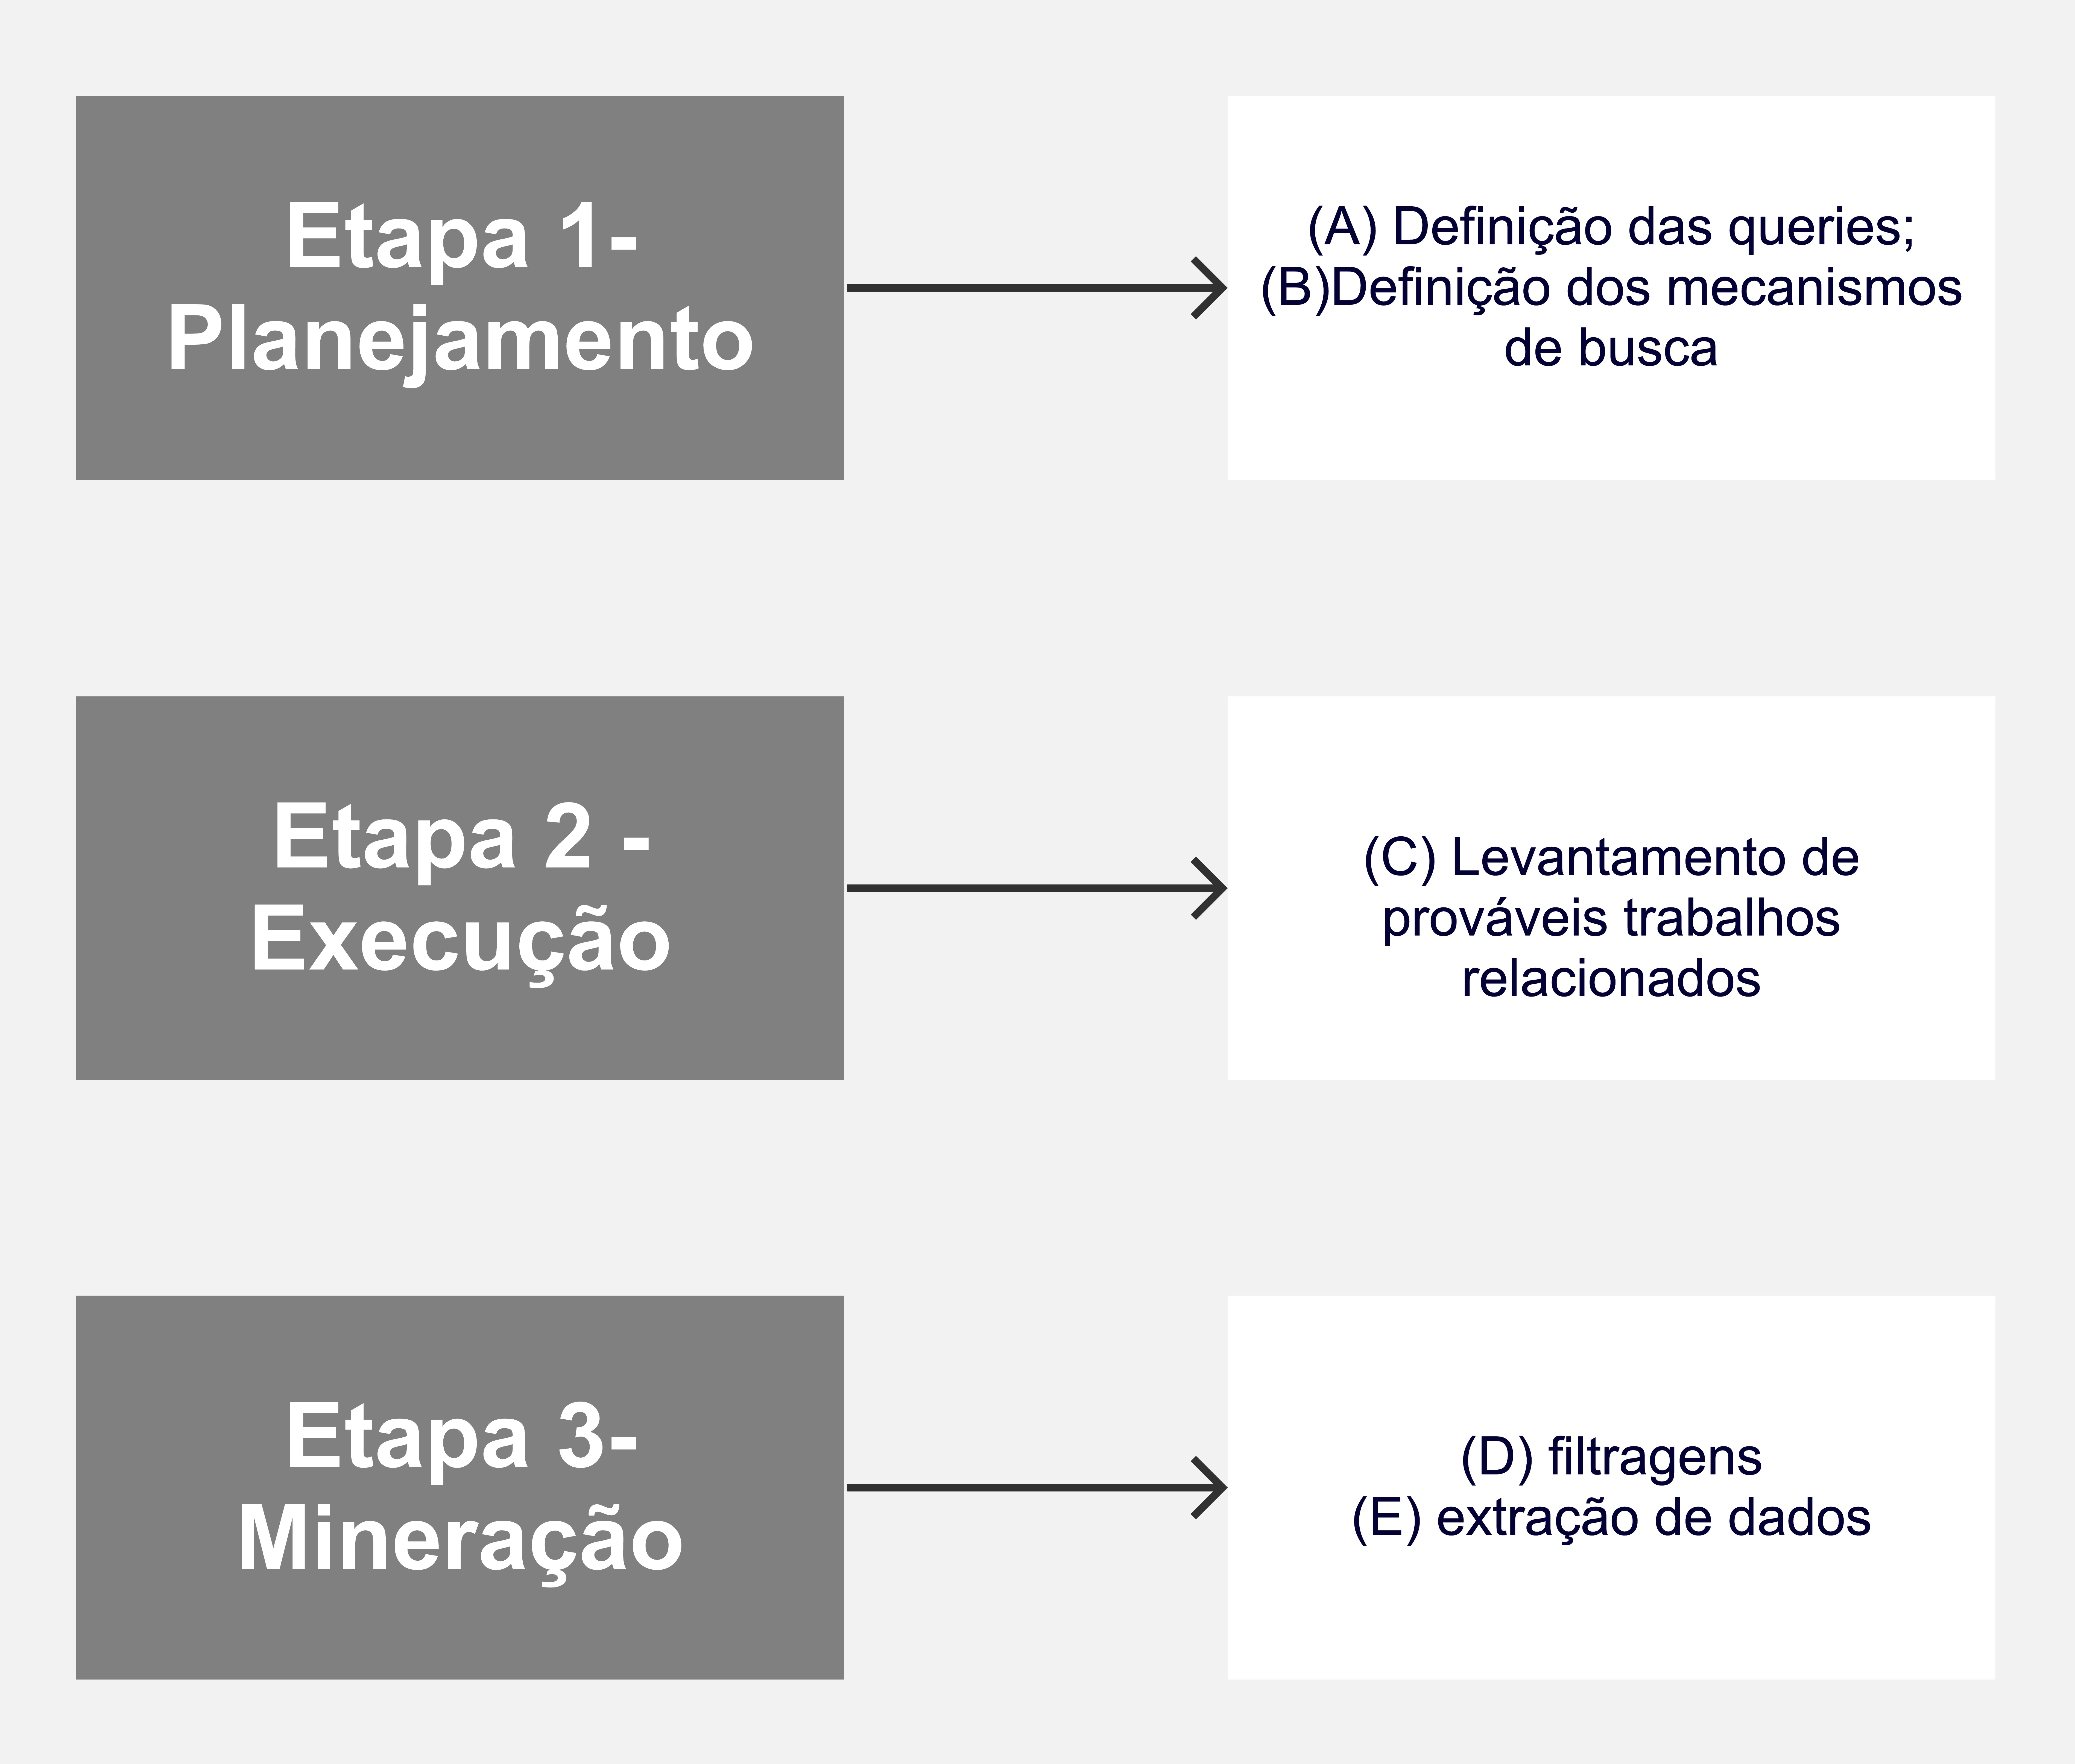
\includegraphics[width=10cm,height=\textwidth,keepaspectratio]{Dissertation//Weslley-Rosalem_Dissertacao-Estudos-Especiais-Quali//2-images/2- Fluxograma mestrado.jpg}
    \newline
    \centering{Fonte: Elaborado pelo autor}
    \label{fig:processo_rev_sistematica}
\end{figure}

As etapas apresentadas na figura \ref{fig:processo_rev_sistematica} são detalhadas a seguir:

\begin{enumerate}
    
    \item As \textit{queries}\footnote{\textit{Queries} são instruções ou expressões usadas para recuperar informações de um banco de dados. Elas são frequentemente escritas em uma linguagem de consulta de banco de dados como SQL.} são \textit{strings}\footnote{\textit{Strings} são sequências de caracteres usadas para representar texto em programação e computação. Elas são fundamentais para o processamento de texto, pesquisa e muitas outras aplicações.}
 que estabelecem critérios para a seleção de artigos. Nesta pesquisa, o foco foi em artigos cujo título ou \textit{keywords}\footnote{\textit{Keywords} são palavras ou frases que resumem o conteúdo principal de um texto, documento ou base de dados. Elas são frequentemente usadas em buscas para encontrar informações relevantes.}
 incluíssem a palavra \textit{AIOPs}. Além disso, restringiu-se o período de publicação entre 2018 e o primeiro semestre de 2023.
    
    \item Dada a reconhecida relevância em Ciência da Computação, especialmente em Redes de Computadores, monitoramento e observabilidade, duas bases de pesquisa científica foram selecionadas: IEEExplore\footnote{https://ieeexplore.ieee.org/} e ACM \textit{Digital Library}\footnote{https://dl.acm.org/}.
    
    \item A execução das \textit{queries} nas bases mencionadas resultou em 80 artigos. A distribuição dos artigos por ano de publicação é ilustrada na Figura \ref{fig:grafico_num_papers}:
      \begin{figure}[H]
    \centering
    \caption{Distribuição dos artigos por ano de publicação.} 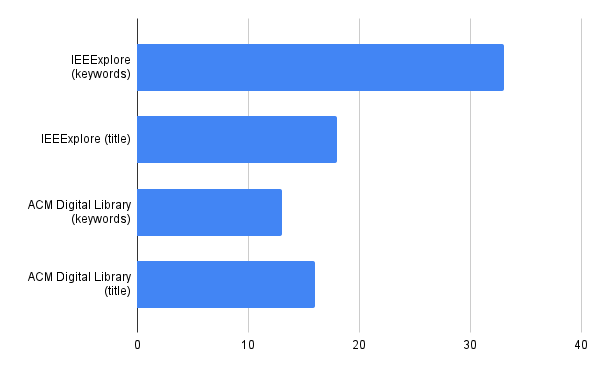
\includegraphics[width=13cm,height=\textwidth,keepaspectratio]{2-images/artigos-bars-horizontal.png}
    \newline \centering{ Fonte: Elaborado pelo autor}\label{fig:grafico_num_papers}
    \end{figure}
    
   \item Durante a filtragem, foram removidos artigos duplicados ou inacessíveis, totalizando 22 duplicados e 2 inacessíveis. Dos 56 artigos remanescentes, 35 não se alinhavam diretamente ao escopo desta dissertação. Portanto, após a filtragem, 21 artigos foram reconhecidos como estreitamente relacionados ao tema proposto. A Figura \ref{fig:grafico_processamento_papers} ilustra este processo:

    \begin{figure}[H]
    \centering
    \caption{Detalhamento do resultado após os processos de filtragem dos artigos.} 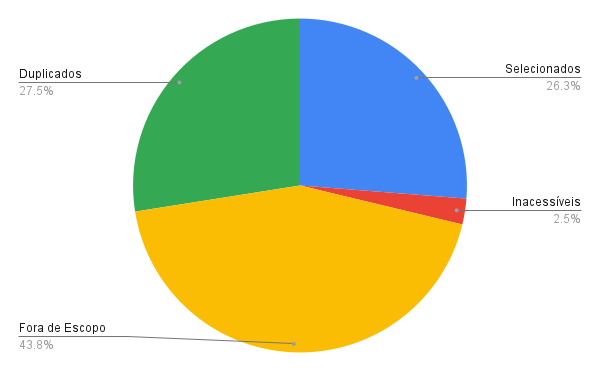
\includegraphics[width=11cm,height=\textwidth,keepaspectratio]{2-images/chart-2.png}
    \newline \centering{ Fonte: Elaborado pelo autor}\label{fig:grafico_processamento_papers}
    \end{figure}    

\item A última etapa envolveu a extração das informações mais relevantes dos artigos selecionados. Para identificar tendências, as seguintes informações foram extraídas:
     \begin{itemize}
         \item Tipo de modelo: técnicas de \textit{machine learning} empregadas ou propostas;
         \item \textit{Dataset}\footnote{Um \textit{dataset} é uma coleção de dados, geralmente apresentada em formato tabular, que serve como entrada para algoritmos de aprendizado de máquina e análise estatística.} : bases de dados utilizadas nos testes;
         \item Arquitetura: arquiteturas propostas;
         \item \textit{Feature selection}\footnote{\textit{Feature Selection} é o processo de selecionar um subconjunto de características relevantes para uso em modelagem. A seleção de características eficaz pode melhorar o desempenho do modelo e reduzir a complexidade computacional.} :
         \item  \textit{features}\footnote{\textit{Features} são variáveis individuais que atuam como entradas em modelos de aprendizado de máquina. Cada feature representa uma dimensão específica de dados que o algoritmo pode usar para aprender.} selecionadas;
         \item Resultados: conclusões alcançadas pelos autores, como RMSE e MAE; e
         \item Metodologia: recursos utilizados na criação do modelo de identificação de anomalias e predição, incluindo linguagens e \textit{softwares}.
     \end{itemize}

\end{enumerate}

Os artigos selecionados foram sintetizados, destacando-se os elementos mais pertinentes ao contexto desta pesquisa. A organização dos estudos foi feita conforme:

\begin{itemize}
    \item Não foram encontrados trabalhos correlatos no ano de 2018. Esta afirmação indica que, após uma busca sistemática na literatura utilizando palavras-chave e critérios específicos, não foram identificados estudos ou publicações relacionadas ao tema da dissertação no ano de 2018;
    \item Trabalhos correlatos de 2019 na Subseção \ref{trab_correlatos_19};
    \item Trabalhos correlatos de 2020 na Subseção \ref{trab_correlatos_20};
    \item Trabalhos correlatos de 2021 na Subseção \ref{trab_correlatos_21};
    \item Trabalhos correlatos de 2022 na Subseção \ref{trab_correlatos_22};
    \item Trabalhos correlatos de 2023 na Subseção \ref{trab_correlatos_23};
\end{itemize}

A Figura \ref{fig:diagrama_detalhado_rev_sistematica} ilustra o processo completo da Revisão Sistemática da Literatura, desde a definição das \textit{queries} até a extração das informações cruciais:


\begin{figure}[H]
\centering
\caption{Procedimento adotado para realização da Revisão Sistemática da Literatura.} 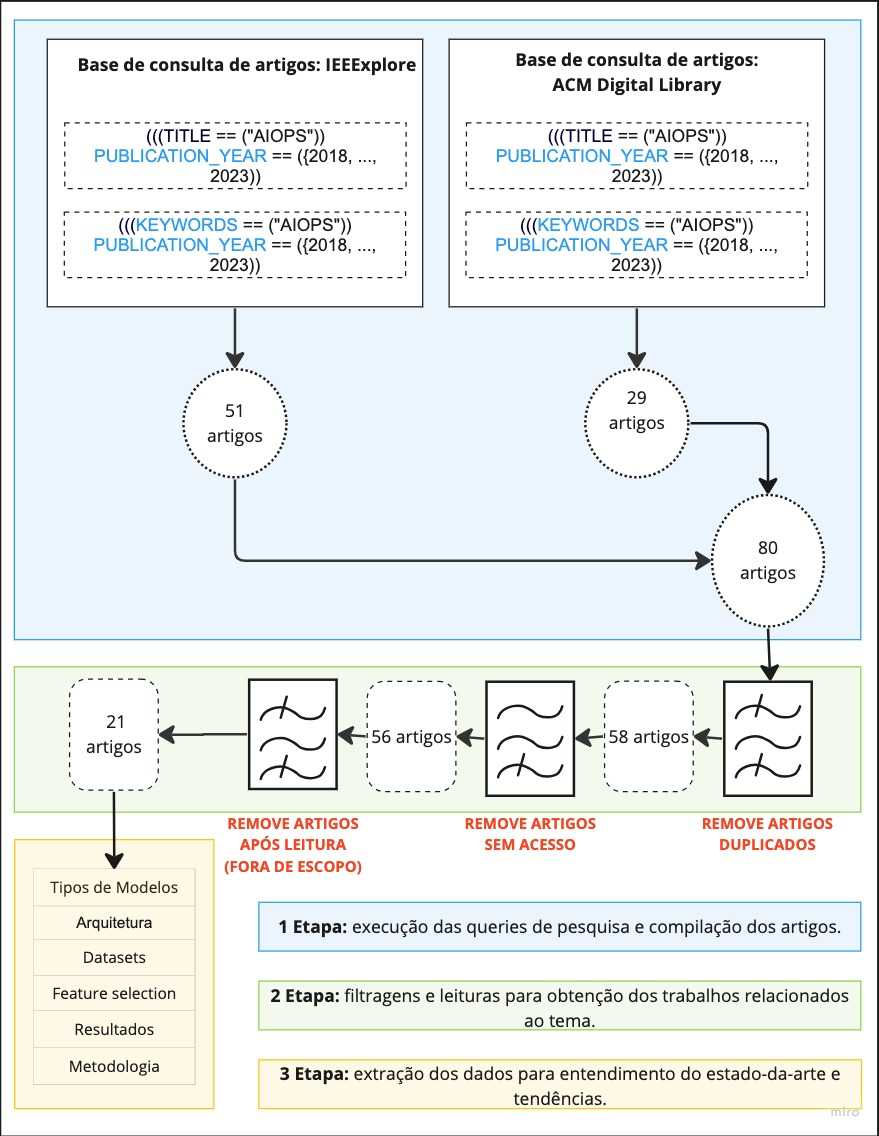
\includegraphics[width=9cm,height=\textwidth,keepaspectratio]{2-images/Fluxograma-papers.png}
\newline \centering{Fonte: Elaborado pelo autor}\label{fig:diagrama_detalhado_rev_sistematica}
\end{figure}    
    

\subsection{Trabalhos Correlatos - ano de 2019}\label{trab_correlatos_19}

No artigo de \cite{8752866}, os autores exploram a aplicação de Inteligência Artificial nas Operações de TI (AIOps) para detectar anomalias com base em registros de \textit{distributed tracing}. Estes registros fornecem informações detalhadas sobre a disponibilidade e o tempo de resposta dos serviços. A abordagem proposta foca na detecção de anomalias no tempo de resposta usando aprendizado não supervisionado. Eles empregam técnicas de modelagem de dados de aprendizado profundo e avaliam a precisão e o desempenho da abordagem em ambientes de teste e produção. A combinação de GRUs (Unidades Recorrentes de Memória) e \textit{autoencoders} variacionais é destacada como uma técnica promissora para modelar séries temporais complexas.

\subsection{Trabalhos Correlatos - ano de 2020}\label{trab_correlatos_20}

O estudo de \cite{9156101} aborda o desafio de monitorar ambientes de TI complexos, que englobam nuvens privadas e públicas, ambientes de IoT, aplicativos e contêineres. Eles destacam a necessidade de um modelo de contexto em AIOps para gerenciar grandes volumes de dados armazenados em diferentes formatos. O \textit{framework} proposto é estruturado em cinco camadas: aquisição, gerenciamento, análise, apresentação de dados e respostas automatizadas. O \textit{Monitoring Resource Model} (MRM) é um componente central desse \textit{framework}. Para a análise de dados, é proposto um modelo de aprendizado de máquina baseado em redes neurais, especificamente o \textit{Long-Short-Term-Memory} (LSTM).

\cite{9311349} discute a importância do aprendizado de máquina, especialmente no contexto de AIOps, para descobrir relacionamentos entre objetos e processos em infraestruturas de TI convergentes. O estudo enfatiza a necessidade de técnicas de aprendizado de máquina para identificar padrões e sequências em grandes volumes de eventos. A arquitetura proposta foca na análise e aprendizado de máquina para processar dados de diversos dispositivos e instrumentos de TI.

O objetivo do estudo apresentado por \cite{9443765} é propor uma rede neural dinâmica para prever fluxos de dados de séries temporais em cenários de AIOps. Os modelos de aprendizado de máquina discutidos incluem \textit{MWNN (Multi-Way Neural Network), WNN (Wavelet Neural Network)} e LSTM. Os dados utilizados durante os testes incluem conjuntos de dados de CPUs com diferentes capacidades. Os resultados mostram uma comparação do consumo de recursos para MWNN, WNN e LSTM quando alcançam o mesmo desempenho.



\subsection{Trabalhos Correlatos - ano de 2021}\label{trab_correlatos_21}

No estudo conduzido por \cite{9516546}, os autores propõem uma abordagem inovadora que combina múltiplos métodos integrados para prever a capacidade de recursos. Utilizando o modelo de aprendizado de máquina LSTM (\textit{Long Short-Term Memory}), o estudo demonstra como, com base nos dados históricos, é possível fornecer previsões precisas sobre o uso de recursos de TI, como CPU, disco rígido e memória. Esta abordagem tem potencial para otimizar a gestão de recursos, garantindo que os sistemas permaneçam estáveis e confiáveis.

\cite{9605403} introduz o conceito de \textit{Machine Reasoning} (MR) e destaca seu papel vital na melhoria das Operações de Inteligência Artificial (AIOps) para Redes Baseadas em Intenções. MR é uma subárea da Inteligência Artificial (IA) que se concentra em capturar e utilizar o conhecimento humano através de linguagens semânticas. Esta abordagem complementa a Aprendizagem de Máquina (ML) ao fornecer inferências precisas baseadas no conhecimento adquirido. O estudo apresenta cenários em que MR em AIOps pode ser utilizado para automatizar e aprimorar a identificação da causa raiz de problemas em redes de computadores.

O artigo de \cite{9678534} apresenta o método AID (\textit{Aggregated Intensity of Dependency}) como uma solução eficiente para prever a intensidade das dependências em sistemas de nuvem em larga escala. Os autores utilizam dados simulados e industriais para testar a eficácia do método proposto. Os resultados mostram que o AID é capaz de medir com precisão a intensidade das dependências, superando outras abordagens comparativas.

\cite{9680514} discute o \textit{design} e a implementação de recursos para migrar dados de sistemas de monitoramento antigos para instâncias do \textit{Prometheus} usando o \textit{framework Ananke}. Além disso, o estudo propõe uma estratégia de dimensionamento automático baseada na previsão de picos de tráfego usando o modelo \textit{Facebook} \textit{Prophet}. A abordagem é voltada para monitorar e modelar aplicações nativas de nuvem, com foco em métricas de desempenho em tempo real e estratégias de otimização.

\subsection{Trabalhos Correlatos - ano de 2022}\label{trab_correlatos_22}

\cite{9492267} introduz o TSAGen, uma ferramenta inovadora de geração de séries temporais. Esta ferramenta permite aos pesquisadores gerar dados sintéticos, fornecendo uma fonte de dados confiável para avaliar o desempenho de algoritmos de detecção de anomalias. O TSAGen foi projetado para enfrentar desafios como a geração de diversas anomalias, ajuste da gravidade das anomalias e controle das características dos KPIs gerados.

No estudo de \cite{9746242}, os autores propõem uma rede neural profunda, a CDX-Net, para previsão de séries temporais multivariadas no contexto de AIOps. A arquitetura proposta do CDX-Net incorpora módulos avançados, como ASPP, SRM, CAM, GRU, transformador e AB, para aprimorar os procedimentos de extração e fusão de características.

\cite{9746416} apresenta uma solução para o Desafio ICASSP-SPGC-2022 AIOps, focando na inferência precisa de combinações em \textit{root cause analysis} (RCA). O documento detalha os desafios encontrados nos dados da competição e propõe uma estrutura robusta para resolver o problema, incluindo a introdução de \textit{TextCNN}.

O estudo de \cite{9789784} propõe uma abordagem para gerar relatórios de falhas legíveis por humanos em sistemas de TIC. A abordagem utiliza o modelo LSTM para séries temporais multivariadas e gera um relatório de falha em formato de texto. Os autores testam a eficácia e o desempenho do método proposto usando dados coletados de um sistema de microsserviços em um \textit{cluster Kubernetes} (k8s).


\cite{9825776} apresenta uma discussão profunda sobre a representação gráfica para o DevOps em aplicações baseadas em aprendizado de máquina, também conhecida como MLOps. Os autores exploram meticulosamente as fases do MLOps, desde o planejamento, onde são identificados o problema a ser resolvido e os dados disponíveis, até a seleção de abordagens de análise de dados e algoritmos adequados. A fase de codificação é destacada, onde o sistema e o código de ML são implementados e validados. A fase de validação é discutida em detalhes, enfatizando a avaliação do desempenho do modelo de ML com novos dados. O artigo também destaca a necessidade imperativa de um processo de MLOps integrado e delinea os desafios associados à adoção prática do MLOps.

\cite{9835411} propõe um framework de dimensionamento automático proativo inovador chamado \textit{RobustScaler}, especialmente projetado para cenários de computação em nuvem. O estudo é direcionado para o desenvolvimento de um \textit{framework} que não apenas gera decisões de mudança e elasticidade, mas também otimiza o equilíbrio entre custo e Qualidade de Serviço (QoS). O modelo proposto é robusto, capaz de lidar com ruídos, dados ausentes e anomalias. O algoritmo de Método dos Multiplicadores de Direção Alternada (ADMM) é usado para treinar o modelo, que captura tanto a periodicidade quanto a estocasticidade das chegadas de consultas. A arquitetura do \textit{framework} é composta por componentes essenciais, como detecção de periodicidade, modelagem histórica de chegadas de consultas, previsão de chegada de consultas e plano de dimensionamento.

\cite{9892264} introduz um \textit{framework} inovador baseado em aprendizado federado, o EFL-WP, projetado especificamente para previsão de carga de trabalho em ambientes inter-nuvem. O \textit{framework} visa colaborar na formação de modelos de \textit{machine learning} para previsão de carga de trabalho, garantindo que informações sensíveis não sejam compartilhadas. Os autores sugerem o uso de modelos LSTM para prever métricas de desempenho, como utilização da CPU e memória. A arquitetura proposta é composta por um coordenador que agenda tarefas de treinamento e orquestra os treinadores, enquanto os treinadores usam seus dados para treinar modelos locais.

\cite{9978983} apresenta o método "\textit{PUTraceAD}" \textit{Positive-Unlabeled}, uma abordagem inovadora para detecção de anomalias em \textit{tracing} de microsserviços. A arquitetura proposta é tripartida, envolvendo \textit{Embedding} de \textit{Span}, Construção de Grafo de Rastros e Treinamento do Modelo. Utilizando uma GNN (\textit{Graph Neural Network}) e aprendizado PU, o método é capaz de detectar anomalias em \textit{tracing} com precisão. O conjunto de dados usado, \textit{TrainTicket}, é um sistema de referência de microsserviços, e os experimentos foram conduzidos em um \textit{cluster Kubernetes}. Os resultados dos experimentos avaliam a eficácia e eficiência do \textit{PUTraceAD}, bem como o impacto de diferentes configurações.

\cite{9985105} discute o Sistema de Gerenciamento de Dependências, ou \textit{Dependency Management System} (DMS), uma solução abrangente para gerenciar dependências de serviços em sistemas em nuvem. O DMS é uma plataforma \textit{end-to-end} que suporta todo o ciclo de vida para garantir a confiabilidade do serviço, desde a implantação inicial até a otimização arquitetural proativa e a mitigação reativa de falhas. Os dados usados nos testes do DMS abrangem uma variedade de fontes, incluindo informações de dependência coletadas de \textit{trancing} distribuído, arquivos de configuração, consultas do orquestrador de serviços e relatórios de dependência de implantação.

\cite{10004053} aborda questões relacionadas à implementação da observabilidade em sistemas de informações hospitalares (HIS). O artigo apresenta uma pesquisa literária detalhada e fornece um resumo abrangente de conceitos relacionados, incluindo definições de monitoramento e HIS, requisitos e soluções em cenários específicos. A arquitetura proposta integra microsserviços e AIOps, com indicadores-chave (KPIs) como qualidade e escala de dados. O documento também oferece sugestões valiosas para os departamentos de TI dos hospitais sobre como abordar essas questões.

\cite{10020986} realiza uma análise detalhada de AIOps na gestão unificada de resiliência de dados em data lakehouses. O artigo propõe soluções inovadoras para prever violações do Recovery Point Objective (RPO) e fornecer sugestões valiosas aos SREs sobre como configurar recursos do sistema para evitar tais violações. Utilizando aprendizado supervisionado em conjunto com análise de séries temporais, o artigo propõe um modelo de aprendizado de máquina que combina métodos de aprendizado online e offline e filtragem de solicitações previstas para garantir a estabilidade das solicitações futuras.



\subsection{Trabalhos Correlatos - ano de 2023}\label{trab_correlatos_23}

%56
Em \cite{10098585}, os autores apresentam uma análise detalhada sobre a implementação de \textit{baselines} utilizando a linguagem de programação \textit{Python}. Eles escolhem a regressão linear como o modelo de aprendizado de máquina para sua análise. O artigo aborda profundamente as questões de pesquisa, o design experimental meticuloso, a aplicação na análise de desempenho e as distribuições de latência. Os autores também discutem o uso de cargas de trabalho que variam continuamente e fornecem \textit{insights} sobre a configuração experimental, destacando a importância de uma abordagem sistemática para garantir resultados precisos e confiáveis.

%57
\cite{10113794} oferece uma visão abrangente do desenvolvimento do sistema de detecção de \textit{outlier} denominado \textit{OutSpot}. Este sistema é especialmente projetado para \textit{datacenters} de alto desempenho e alta criticidade, que são primordialmente responsáveis pelo fornecimento de \textit{streaming} de vídeos. O principal objetivo do sistema é detectar \textit{outliers} nos KPIs coletados desses \textit{datacenters}. O modelo de ML adotado é uma combinação inovadora de \textit{Hierarchical Agglomerative Clustering} (HAC) com Conditional Variational Autoencoder (CVAE). O HAC é utilizado para agrupar os KPIs com base em seus padrões distintos. Posteriormente, as informações de agrupamento de cada KPI são incorporadas ao método. Esta abordagem integrada permite que o \textit{OutSpot} detecte \textit{outliers} para KPIs em larga escala, mesmo quando esses KPIs apresentam padrões variados. A arquitetura proposta para o \textit{OutSpot} é meticulosa, dividindo os conjuntos de dados coletados em conjuntos de treinamento e teste. O conjunto de treinamento é composto por dados coletados ao longo dos primeiros 7 dias, enquanto o conjunto de teste contém dados do último dia. Este último conjunto é rotulado cuidadosamente por operadores experientes utilizando uma ferramenta desenvolvida pelos próprios autores. O processo de rotulação dos \textit{outliers} é rigoroso, envolvendo três operadores, e a decisão final é tomada apenas quando os rótulos fornecidos por eles divergem.



% Please add the following required packages to your document preamble:
% \usepackage{longtable}
% Note: It may be necessary to compile the document several times to get a multi-page table to line up properly
\begin{longtable}{|p{2.5cm}|p{4cm}|p{8cm}|}
\caption{Características da análise sistemática da literatura}
\label{tab:res-anali-sistematica}\\
\hline
\textbf{Ano de Publicação} & \textbf{Autores}         & \textbf{Tópico Principal}                                                                              \\ \hline
\endfirsthead
%
\endhead
%
2019              & \cite{8752866}  & Detecção de anomalias usando \textit{Distributed Tracing} e \textit{Deep Learning} em AIOps                     \\ \hline
2020              & \cite{9156101}  & Monitoramento de ambiente de TI complexo com modelo de contexto                               \\ \hline
2020              & \cite{9311349}  & Redução de incidentes em infraestruturas de TI convergentes através de aprendizado de máquina \\ \hline
2020              & \cite{9443765}  & Previsão de fluxos de dados de séries temporais em cenários de AIOps                          \\ \hline
2021              & \cite{9516546}  & Previsão da capacidade de recursos usando LSTM                                                \\ \hline
2021              & \cite{9605403}  & Melhoria das Operações de IA para Redes Baseadas em Intenções usando \textit{Machine Reasoning}        \\ \hline
2021              & \cite{9678534}  & Previsão da intensidade de dependências em sistemas em nuvem                                  \\ \hline
2021              & \cite{9680514}  & Migração de dados de sistemas de monitoramento antigos para instâncias do \textit{Prometheus}          \\ \hline
2022              & \cite{9492267}  & Geração de séries temporais para avaliação de algoritmos de detecção de anomalias             \\ \hline
2022              & \cite{9746242}  & Previsão de séries temporais multivariadas em AIOps                                           \\ \hline
2022              & \cite{9746416}  & Inferência precisa de combinações em \textit{root} cause \textit{analysis}                                      \\ \hline
2022              & \cite{9789784}  & Geração de relatórios de falhas legíveis por humanos em sistemas de TIC                       \\ \hline
2022              & \cite{9825776}  & Representação gráfica para o \textit{DevOps}\footnote{\textit{DevOps} é uma filosofia e prática de engenharia de software que visa unificar o desenvolvimento de software (\textit{Dev}) e a operação de software (\textit{Ops}). O principal objetivo de DevOps é encurtar o ciclo de vida do desenvolvimento de sistemas, proporcionando entrega contínua de alta qualidade, e, assim, melhorar a colaboração e a comunicação entre as equipes de desenvolvimento e operações. *DevOps* integra métodos ágeis, automação, integração contínua, entrega contínua e monitoramento contínuo do software em operação.}
 em aplicações baseadas em aprendizado de máquina (MLOps)  \\ \hline
2022              & \cite{9835411}  & \textit{Framework} de dimensionamento automático proativo para computação em nuvem                     \\ \hline
2022              & \cite{9892264}  & Previsão de carga de trabalho em ambientes de inter-nuvem usando aprendizado federado         \\ \hline
2022              & \cite{9978983}  & Detecção de anomalias em \textit{tracing} de microsserviços usando GNN e aprendizado PU                \\ \hline
2022              & \cite{9985105}  & Gerenciamento de dependências de serviços em sistemas em nuvem                                \\ \hline
2022              & \cite{10004053} & Implementação da observabilidade em sistemas de informações hospitalares (HIS)                \\ \hline
2022              & \cite{10020986} & Gestão unificada de resiliência de dados em data \textit{lakehouses}                                   \\ \hline
2023              & \cite{10098585} & Implementação de \textit{baselines} usando \textit{Python} e regressão linear                                   \\ \hline
2023              & \cite{10113794} & Detecção de \textit{outlier} para \textit{datacenters} com alto nível de desempenho e alta criticidade          \\ \hline
\end{longtable}


\section{Arquitetura \textit{Transformer}} \label{sec-arquitetura-transformer}

A arquitetura \textit{Transformer} foi pioneiramente introduzida no artigo \textit{"Attention Is All You Need"} por \cite{vaswani2017attention}. Esta arquitetura representou uma mudança paradigmática no processamento de sequências. Ao contrário dos modelos tradicionais, como as redes neurais convolucionais (CNNs) e as redes neurais recorrentes (RNNs), especialmente em tarefas de processamento de linguagem natural (PLN),  eliminando a necessidade de recorrência e convoluções, centrando-se exclusivamente em mecanismos de atenção, que permite ao modelo ponderar diferentes segmentos da entrada com base em sua relevância para a tarefa em questão, e desta maneira para discernir dependências contextuais entre os dados de uma maneira mais eficiente e escalável. 


As redes neurais \textit{feed-forward} formam a base da arquitetura \textit{Transformer}, que em sua essência é composto por dois componentes principais: um codificador (\textit{encoder}) e um decodificador (\textit{decoder}). Cada um desses componentes é uma pilha de camadas idênticas que contêm sub-camadas \textit{feed-forward}. Sua estrutura é explicada nas subseções seguintes.

\subsection{Redes Neurais Feed-forward}
As redes neurais \textit{feed-forward} dentro das sub-camadas do \textit{Transformer} são relativamente simples, consistindo geralmente em duas camadas lineares com uma ativação não-linear entre elas. A função destas redes \textit{feed-forward} é transformar os dados de forma independente em cada posição.

\subsection{Mecanismo de Atenção}
O principal elemento desta arquitetura é o mecanismo de "atenção multi-cabeça". Este mecanismo permite que o modelo pondere diferentes segmentos da sequência de entrada de maneira variável, dependendo da relevância contextual de cada segmento ao gerar cada componente da sequência de saída \cite{vaswani2017attention}. Esse foco adaptativo permite que o modelo capture nuances e dependências sutis em dados sequenciais. Matematicamente, o mecanismo de atenção é formulado como:

\[
\text{Attention}(Q, K, V) = \text{softmax}\left(\frac{QK^T}{\sqrt{d_k}}\right) V
\]

Nesta formulação, \(Q\), \(K\), e \(V\) representam as matrizes de consulta, chave e valor, respectivamente. \(d_k\) denota a dimensionalidade das chaves. Este mecanismo sofisticado permite que o modelo \textit{Transformer} aloque atenção diferenciada a diferentes segmentos da entrada, otimizando sua capacidade de modelar relações complexas nos dados \cite{vaswani2017attention}.

\subsection{Codificador e Decodificador}
O codificador é a primeira etapa da arquitetura \textit{Transformer} e é responsável por processar e transformar a entrada em uma representação contínua e abstrata. Esta representação é então passada para o decodificador, que a utiliza para gerar a saída desejada. Ambos, codificador e decodificador, são compostos por múltiplas camadas que contêm mecanismos de atenção e redes neurais \textit{feed-forward}, permitindo uma modelagem profunda e abrangente dos dados.

Cada camada no codificador contém duas sub-camadas: a primeira é a atenção multi-cabeça e a segunda é uma rede neural \textit{feed-forward} simples. A rede \textit{feed-forward} é aplicada separadamente e de forma idêntica a cada posição, ou seja, é a mesma operação em todos os elementos da sequência, mas é aplicada de forma independente para cada um.

Além das duas sub-camadas presentes no codificador, cada camada do decodificador possui uma terceira sub-camada que realiza atenção multi-cabeça sobre a saída do codificador. Esta atenção inter-camadas ajuda o decodificador a focar em partes relevantes da entrada ao gerar a saída.


\subsection{Codificação Posicional}
Uma característica distintiva do \textit{Transformer} é a sua capacidade de processar sequências sem depender de recorrência. Para compensar a ausência de uma noção inerente de ordem, o modelo utiliza codificações posicionais. Estas codificações são adicionadas aos \textit{embeddings} de entrada, garantindo que o modelo possa considerar a posição relativa de cada elemento na sequência \cite{vaswani2017attention}.

\subsection{Normalização de Camada}
Para garantir a estabilidade e a eficiência do treinamento, cada sub-camada dentro dos codificadores e decodificadores é acompanhada por uma normalização de camada. Este processo ajusta e estabiliza as ativações, permitindo uma convergência mais rápida e um treinamento mais estável \cite{ba2016layer}. Uma representação simplificada dessa formulação, pode ser dada por:
\[
\text{LayerNorm}(x + \text{Sublayer}(x))
\]

Nesta equação, \(\text{\textit{Sublayer}}(x)\) representa a saída de uma das sub-camadas, como a atenção multi-cabeça ou a rede neural \textit{feed-forward}.


\subsection{Pseudo-código}
Para uma compreensão detalhada e mais profunda da implementação do \textit{Transformer}, um pseudo-código detalhado é fornecido no apêndice \ref{appendix:a}.

\subsection{Desafios e Limitações}
Apesar de suas inúmeras vantagens, o \textit{Transformer} apresenta desafios. Sua complexidade computacional, especialmente em modelos de grande escala, pode ser proibitiva em certos cenários. Além disso, embora o mecanismo de atenção ofereça algum grau de visibilidade sobre o funcionamento do modelo, ele não garante uma interpretabilidade completa, o que pode ser um obstáculo em aplicações que exigem transparência total \cite{jiang2019attention}.


\section{Análise Preditiva com \textit{Transformer}} \label{cap-anal-pre-trans-ts}

A análise preditiva de séries temporais é uma área de pesquisa em rápido crescimento, com aplicações em diversos domínios, desde o setor financeiro até operações de TI. Este estudo adota a arquitetura \textit{Transformer}, que, embora originalmente projetada para tarefas de processamento de linguagem natural \cite{vaswani2017attention}, demonstrou uma capacidade notável de modelar dependências temporais em séries temporais \cite{lim2019temporal}.


\subsection{Arquitetura \textit{Transformer} em Séries Temporais}
O \textit{Time Series Transformer} (TST), é uma extensão especializada do \textit{Transformer}, adaptado para lidar com as nuances e características específicas das séries temporais \cite{lim2019temporal}. Mantendo o mecanismo de atenção, o TST é capaz de capturar dependências temporais em múltiplas escalas, tornando-o ideal para modelar e analisar sequências temporais.

A eficácia do TST é fortemente influenciada pela seleção apropriada de hiperparâmetros. A escolha do número de camadas, dimensão do modelo e número de cabeças de atenção é crucial. Estes parâmetros devem ser meticulosamente ajustados conforme a natureza dos dados e o problema específico para garantir o desempenho ótimo do modelo.

Quando aplicado a métricas de séries temporais, como as armazenadas em sistemas como o \textit{Prometheus}, o TST tem o potencial de discernir padrões intrincados e dependências temporais, facilitando a identificação de anomalias, sazonalidades e a previsão de tendências futuras.  

\subsection{Inteligência Artificial}
A Inteligência Artificial (IA) é uma disciplina interdisciplinar que aspira a criar máquinas capazes de emular comportamentos inteligentes humanos \cite{russell2016artificial}. A IA engloba habilidades como aprendizado a partir de experiências, compreensão de linguagem natural, reconhecimento de padrões e tomada de decisões autônomas. Ela é o resultado da convergência de campos como ciência da computação, matemática, psicologia, neurociência e linguística.

Nos últimos anos, a IA tem experimentado avanços significativos, impulsionados por melhorias em algoritmos, capacidades computacionais avançadas e a disponibilidade de grandes volumes de dados \cite{poole2017artificial}.

O aprendizado de máquina, uma subárea proeminente da IA, foca em desenvolver algoritmos que aprimorem seu desempenho com base nos dados fornecidos \cite{mitchell1997machine}. O aprendizado profundo, uma subdivisão do aprendizado de máquina, tem se destacado em tarefas complexas, como reconhecimento de imagens e processamento de linguagem natural, devido à sua capacidade de modelar relações intrincadas em grandes conjuntos de dados \cite{lecun2015deep}.

\subsection{AIOps}
AIOps, uma abreviação para Inteligência Artificial para Operações de TI, é um conceito introduzido pelo \textit{Gartner}, que se refere à integração de técnicas de IA nas operações de TI \cite{gardner2017artificial}. AIOps visa aprimorar e automatizar aspectos das operações de TI, como monitoramento, gerenciamento e análise de dados, através da combinação de \textit{big data} e aprendizado de máquina.

Com AIOps, as operações de TI podem transitar de uma abordagem reativa para uma proativa. Isso significa que, em vez de apenas responder a problemas após sua ocorrência, é possível antecipar e prevenir problemas, otimizando a eficiência e confiabilidade das operações de TI \cite{sill2019aiops}.

\subsection{Séries Temporais e Prometheus}
Séries temporais são conjuntos ordenados de dados coletados em intervalos sequenciais e regulares \cite{shumway2017time}. No contexto de TI, elas são essenciais para monitorar e otimizar sistemas, com métricas como uso de CPU, memória e tráfego de rede sendo essenciais para garantir a estabilidade dos sistemas.

Séries temporais são conjuntos de dados organizados em intervalos sequenciais e regulares, com cada ponto de dados associado a um carimbo de data/hora específico. Esses dados são fundamentais para realizar análises de tendências, detecção de anomalias e previsões futuras, especialmente em ambientes dinâmicos onde os estados do sistema estão sujeitos a flutuações frequentes.

O \textit{Prometheus} é uma solução de monitoramento e alerta de código aberto, foi desenvolvida pela empresa \textit{SoundCloud} e é atualmente mantida pela \textit{Cloud Native Computing Foundation} \cite{brazil2019prometheus}. Sua robustez e escalabilidade o tornam uma escolha popular para monitorar ambientes de nuvem nativa, especialmente devido à sua integração com o \textit{Kubernetes}\footnote{\textit{Kubernetes} é um sistema de orquestração de contêineres de código aberto que automatiza a implantação, o escalonamento e a gestão de aplicações em contêineres. Desenvolvido originalmente pelo Google e agora mantido pela \textit{Cloud Native Computing Foundation}, *Kubernetes* fornece um framework para executar sistemas distribuídos resilientes, permitindo a escalabilidade sem aumentar a carga de trabalho da equipe de operações de TI.}.

No contexto dos ambientes de TI modernos, a avaliação exaustiva do desempenho e da confiabilidade dos sistemas e aplicações é imperativa para assegurar tanto a satisfação do usuário quanto a continuidade operacional. Entre as diversas ferramentas e técnicas disponíveis para o monitoramento eficiente dos sistemas, a análise de séries temporais de métricas emergiu como um dos métodos mais eficazes e confiáveis.


\subsection{Treinamento e Otimização}
O treinamento do modelo \textit{Transformer} é uma etapa meticulosa, que envolve alimentar o modelo com janelas de dados temporais, e, ajustar seus parâmetros para minimizar o erro nas previsões. Durante esta fase, vários hiperparâmetros\footnote{Hiperparâmetros são parâmetros que não são aprendidos pelo modelo durante o treinamento, mas são definidos a priori para estruturar o modelo de aprendizado de máquina. Eles incluem, por exemplo, a taxa de aprendizado, o tamanho do lote e o número de épocas em redes neurais. A escolha adequada dos hiperparâmetros é crucial para o desempenho do modelo.} são customizados, como o número de camadas de atenção, a dimensionalidade dos vetores de atenção e o número de "cabeças de atenção", serão otimizados. Para isso, serão empregadas técnicas avançadas de busca de hiperparâmetros, como \textit{grid search}\footnote{\textit{Grid Search} é uma técnica de otimização de hiperparâmetros que envolve a exploração exaustiva de um conjunto predefinido de hiperparâmetros. O algoritmo treina um modelo para cada combinação de hiperparâmetros e seleciona a configuração que oferece o melhor desempenho no conjunto de validação. Embora eficaz, o \textit{Grid Search} pode ser computacionalmente intensivo e demorado.} e \textit{Bayesian optimization}\footnote{\textit{Bayesian Optimization} é uma estratégia para a otimização global de funções custosas e sem ruído. Diferentemente do \textit{Grid Search}, que faz uma busca exaustiva, a \textit{Bayesian Optimization} usa um modelo probabilístico para prever a qualidade de diferentes configurações de hiperparâmetros.}, que exploram o espaço de hiperparâmetros para encontrar a combinação ideal que resulta no melhor desempenho do modelo \cite{bergstra2012random}.

\subsection{Métricas}
A avaliação meticulosa do desempenho do modelo é fundamental para entender sua eficácia em tarefas de previsão e detecção de anomalias. Para isso, serão empregadas métricas quantitativas robustas, como \textit{Root Mean Squared Error} (RMSE) e \textit{Mean Absolute Error} (MAE), que fornecem insights valiosos sobre a precisão e a robustez do modelo.

\subsubsection{Root Mean Squared Error (RMSE)}

O RMSE é uma métrica de avaliação de desempenho que mede a média das diferenças quadradas entre os valores previstos e os valores reais. O RMSE é sensível a \textit{outliers} e penaliza erros maiores mais severamente do que erros menores. É frequentemente usado em tarefas de regressão e previsão por ser uma métrica quantitativa que avalia a magnitude dos erros entre as previsões do modelo e os valores reais. É calculado como:

\[
RMSE = \sqrt{\frac{\Sigma (P_i - O_i)^2}{n}}
\]

Nesta formulação, \(P_i\) e \(O_i\) representam os valores previstos e observados, respectivamente, e \(n\) é o número total de observações. O RMSE é particularmente sensível a \textit{outliers} e penaliza erros maiores de forma mais severa do que erros menores. Isso o torna uma métrica valiosa em contextos onde erros grandes são particularmente indesejáveis \cite{willmott2005advantages}.

\subsubsection{Mean Absolute Error (MAE)}

O MAE é uma métrica de avaliação de desempenho que calcula a média das diferenças absolutas entre os valores previstos e os valores reais. Diferentemente do RMSE, o MAE é menos sensível a outliers e pode ser mais apropriado quando erros grandes não são tão críticos, por ser uma métrica que quantifica a média das diferenças absolutas entre os valores previstos pelo modelo e os valores reais. É formulado como:

\[
MAE = \frac{\Sigma | P_i - O_i|}{n}
\]

Semelhante ao RMSE, \(P_i\) e \(O_i\) representam os valores previstos e observados, respectivamente, e \(n\) é o número total de observações. O MAE é menos sensível a \textit{outliers} do que o RMSE e, portanto, fornece uma avaliação mais robusta do desempenho do modelo, especialmente em contextos onde \textit{outliers} são menos críticos \cite{willmott2005advantages}.

\subsubsection{Relevância das Métricas}

Ambas as métricas, RMSE e MAE, são de suma importância para este estudo, pois oferecem diferentes perspectivas sobre o desempenho do modelo. Enquanto o RMSE é valioso para avaliar o impacto de erros grandes, o MAE fornece uma avaliação mais equilibrada e robusta, minimizando o impacto de \textit{outliers}\footnote{\textit{Outliers} são observações em um conjunto de dados que se desviam significativamente das outras observações. Eles são anômalos e podem indicar uma variabilidade incomum, erro de medição ou entrada de dados, ou uma mudança genuína no processo subjacente. Tecnicamente, um \textit{outlier} é um ponto de dado que difere substancialmente do resto do conjunto de dados}.

\chapter{Metodologia} \label{Cap_metodologia}

Esta pesquisa adota uma metodologia sofisticada, utilizando a arquitetura \textit{Transformer} para a análise meticulosa de séries temporais, especificamente métricas de desempenho de sistemas de TI, coletadas através do sistema \textit{Prometheus}. Originalmente concebida para tarefas de processamento de linguagem natural, a arquitetura \textit{Transformer} foi adaptada com sucesso para séries temporais, exibindo uma capacidade notável em diversas tarefas, incluindo previsão precisa e detecção de anomalias complexas.

O \textit{Prometheus} será utilizado para a coleta de dados, uma escolha motivada pela sua robustez, eficiência e adoção generalizada em ambientes de nuvem nativa. Este sistema é capaz de armazenar métricas de séries temporais de vários componentes de um sistema de TI, incluindo, mas não se limitando a, uso de CPU, memória, velocidade de escrita e leitura em disco, quantidade de acessos simultâneo, velocidade no tempo de resposta, e tráfego de rede.

A metodologia empregada compreende várias etapas críticas. Inicialmente, os dados coletados passarão por um pré-processamento rigoroso para convertê-los em um formato compatível para serem introduzidos no modelo \textit{Transformer}. Posteriormente, o modelo será treinado com o objetivo de aprender representações profundas e abstratas das métricas de desempenho, juntamente com suas dependências temporais intrínsecas. A eficácia do modelo será avaliada meticulosamente através de técnicas de validação cruzada, juntamente com uma comparação detalhada com \textit{benchmarks} estabelecidos.

\section{Conjunto de Dados}

O conjunto de dados utilizado nesta pesquisa é único, composto por dados coletados de um ambiente de TI real, utilizando o \textit{Prometheus}. A decisão de empregar dados reais é instrumental para avaliar a eficácia do modelo em condições autênticas, uma etapa crucial para compreender tanto a aplicabilidade quanto ás possíveis limitações da abordagem proposta. 

Este \textit{dataset}\footnote{Um \textit{dataset}, ou conjunto de dados, é uma coleção de dados geralmente apresentada em forma tabular, onde cada linha representa uma observação ou instância, e cada coluna representa uma variável, característica ou atributo dessas observações. Os \textit{datasets} são fundamentais em diversas áreas como ciência da computação, estatística, aprendizado de máquina, e análise de dados, fornecendo a base sobre a qual análises são realizadas e decisões são tomadas.} específico inclui dados históricos derivados de um servidor \textit{web}, com métricas críticas relacionadas ao uso e consumo de recursos, como memória, CPU, disco e rede, todas coletadas em tempo real e meticulosamente armazenadas em formato de série temporal. Todas monitoradas ao longo de um período de trinta dias dias. Essas métricas são frequentemente empregadas em estudos de séries temporais em contextos de TI, devido à sua relevância direta e impacto no desempenho geral do sistema. Mais detalhes sobre este conjunto de dados, pode ser obtido através do repositório no \textit{\href{https://github.com/weslleyrosalem/dissertacao/tree/main/Experiments/data}{Github}}.

\begin{table}[h!]
    \centering
    \caption{Características do conjunto de dados escolhido}
    \begin{tabular}{|c|c|}
        \hline
        \textbf{Feature} & \textbf{Descrição} \\
        \hline
        timestamp & Data e hora da medição \\
        \hline
        cpu\_usage & Percentual de uso da CPU \\
        \hline
        memory\_usage & Uso de memória em bytes \\
        \hline
        network\_latency & Latência de rede em milissegundos \\
        \hline
        network\_traffic & Tráfego de rede em bits por segundo \\
        \hline
    \end{tabular}
    \label{tab:dataset_features}
\end{table}


\section{Carregamento e Pré-processamento de Dados de Séries Temporais}

A fase de carregamento e pré-processamento de dados  é crítica e precede a modelagem, essencial para garantir que o modelo \textit{Transformer} possa interpretar e aprender efetivamente a partir das séries temporais obtidas via \textit{Prometheus}. As séries temporais apresentam desafios únicos devido à sua natureza, e vários aspectos cruciais devem ser meticulosamente abordados durante o pré-processamento.

Além disso, as séries temporais coletadas precisarão ser normalizadas. A normalização é um processo que ajusta os valores medidos em diferentes escalas para uma noção comum, e é vital para o treinamento eficiente do modelo \textit{Transformer}. Isso se deve ao fato de que a arquitetura \textit{Transformer} emprega mecanismos de atenção autorregressiva, que são altamente sensíveis às variações na escala dos dados de entrada. Comumente, os dados são reescalados para ter uma média de zero e um desvio padrão de um, uma técnica conhecida como padronização, que será explorada durante esta fase.

A segmentação dos dados em janelas temporais é outra etapa crucial no pré-processamento. Modelos de séries temporais, incluindo o \textit{Transformer}, operam sobre segmentos ou janelas de dados. A segmentação adequada é essencial para capturar as dependências temporais inerentes aos dados, permitindo que o modelo aprenda e modele efetivamente as relações temporais subjacentes.

Por fim, a divisão dos dados em conjuntos distintos de treinamento e teste é fundamental. Esta divisão permite que o modelo seja treinado, validado e testado em diferentes subconjuntos de dados, garantindo uma avaliação robusta e imparcial do seu desempenho. Importante ressaltar que essa divisão será realizada de forma a preservar a integridade e a ordem temporal dos dados, garantindo que o modelo seja exposto a uma representação autêntica das relações temporais nos dados, todos detalhes estão descritos nas subseções a seguir:

\subsection{Carregamento de Dados}

A inicialização do processo de análise de dados é realizada através do carregamento dos mesmos. Neste estudo, a função \textit{read\_pickle} do pacote \textit{pandas} foi empregada para carregar dados de séries temporais armazenados em formato de serialização (\textit{Python pickle}). Esta metodologia é eficiente para a recuperação de dados complexos, mantendo a integridade e a estrutura original. Os dados são, então, carregados em uma estrutura \textit{DataFrame}, facilitando a manipulação e análise subsequente.

\subsection{Pré-processamento de Dados}

O pré-processamento de dados de séries temporais é fundamental para garantir a precisão nas análises subsequentes. As etapas de pré-processamento neste estudo incluem:

\subsubsection{Reamostragem Temporal}
Utiliza-se a função \textit{resample} do \textit{pandas} para a reamostragem dos dados em intervalos de 30 minutos. Esta abordagem padroniza a frequência dos dados, compensando possíveis coletas em intervalos irregulares. A média dos valores em cada intervalo de 30 minutos é calculada, resultando em uma representação mais consistente da série temporal.

\subsubsection{Divisão em Conjuntos de Treino e Teste}
Os dados são divididos em conjuntos de treino e teste, respeitando a ordem cronológica para manter as dependências temporais. Os dados anteriores a "2021-02-07" são alocados como conjunto de treino, enquanto os dados a partir de "2021-02-08" constituem o conjunto de teste.

\subsubsection{Normalização dos Dados}
A normalização é implementada utilizando o \textit{MinMaxScaler} do \textit{scikit-learn}, escalando os dados para um intervalo entre 0 e 1. O escalador é ajustado ao conjunto de treino para aprender os parâmetros de escala e, em seguida, aplicado tanto ao conjunto de treinos quanto ao de testes.

Estas etapas são cruciais para assegurar a qualidade e a consistência dos dados, permitindo análises precisas e a aplicação efetiva de modelos de aprendizado de máquina em séries temporais.


\section{Estrutura do modelo}
A seguir é documentado os detalhes da estrutura do modelo proposto, e como a arquitetura \textit{Transformer} está sendo empregada para trabalhar com dados de série temporal, seu algoritmo pode ser encontrado tanto no apêndice \ref{appendix:model-implementation} quanto no \href{https://github.com/weslleyrosalem/dissertacao}{\textit{Github}}.

\subsection{Construção do Modelo}
A arquitetura do modelo é baseada no \textit{Transformer}, construído utilizando a função \textit{build\_model} do módulo \textit{model}. Esta função configura uma rede de atenção multi-cabeça (\textit{MultiHeadAttention}), seguida por camadas de normalização (\textit{LayerNormalization}) e convolucionais 1D (\textit{Conv1D}) para processar sequências temporais. Os hiperparâmetros relevantes incluem o tamanho da cabeça da atenção (\textit{head\_size})\footnote{Define o tamanho de cada cabeça na camada de atenção multi-cabeça do \textit{Transformer}. Em modelos de atenção, '\textit{head\_size}' refere-se à dimensão de cada cabeça de atenção individual, sendo um fator crucial para determinar a capacidade do modelo de capturar diferentes aspectos das sequências de entrada}, o número de cabeças (\textit{num\_heads})\footnote{Especifica o número de cabeças na camada de atenção multi-cabeça. O parâmetro '\textit{num\_heads}' é importante para a diversificação da atenção do modelo, permitindo que ele se concentre em diferentes partes da sequência de entrada simultaneamente.}, a dimensão \textit{feed-forward} (\textit{ff\_dim})\footnote{Representa a dimensão da camada \textit{feed-forward} no \textit{Transformer}. Este parâmetro determina o tamanho da camada totalmente conectada que segue a camada de atenção, sendo essencial para a capacidade do modelo de aprender representações complexas.} e a taxa de \textit{dropout} (\textit{dropout\_rate})\footnote{Indica a taxa de \textit{dropout} usada nas camadas do modelo. \textit{Dropout} é uma técnica de regularização usada para prevenir o overfitting, onde uma fração dos neurônios é aleatoriamente desativada durante o treinamento.}. Regularizadores L2 são aplicados nas camadas convolucionais para mitigar o \textit{overfitting}. O modelo é finalizado com uma camada densa para a predição de saída.

\subsection{Treinamento e Avaliação do Modelo}
O treinamento do modelo é realizado pela função \textit{train\_model}, que emprega a função \textit{fit} do \textit{TensorFlow} para ajustar o modelo aos dados de treino. Os parâmetros de treinamento incluem o tamanho do lote (\textit{batch\_size})\footnote{Específica o tamanho do lote para o treinamento do modelo. O '\textit{batch\_size}' afeta diretamente a eficiência do treinamento e a estabilidade do gradiente durante a otimização.} e o número de épocas (\textit{epochs})\footnote{Determina o número de épocas, ou ciclos completos através do conjunto de dados, para o treinamento do modelo. O número de épocas é crucial para garantir que o modelo tenha tempo suficiente para aprender efetivamente dos dados.}. A avaliação do modelo, conduzida pela função \textit{evaluate\_model}, envolve a geração de previsões tanto para os conjuntos de treino quanto de teste, usando a função \textit{predict} do \textit{TensorFlow}. As previsões são então escaladas novamente para sua forma original usando o \textit{MinMaxScaler}. O erro absoluto médio (MAE) é calculado entre as previsões e os valores reais de teste, ajustando-se o tamanho dos \textit{arrays} de previsão e real para garantir a consistência na comparação.

\subsection{Busca de Hiperparâmetros}
A busca de hiperparâmetros é conduzida por um método de pesquisa aleatória, implementado no arquivo \textit{main\_random\_loop.py}. Este método itera sobre um espaço de parâmetros pré-definido, que inclui os passos da sequência (\textit{n\_steps})\footnote{Refere-se ao número de passos (ou intervalos de tempo) considerados na entrada do modelo. Este parâmetro é vital para definir o contexto temporal que o modelo usa para fazer previsões.}, tamanho da cabeça da atenção, número de cabeças, dimensão \textit{feed-forward}, taxa de \textit{dropout}, taxa de aprendizado (\textit{learning\_rate})\footnote{Define a taxa de aprendizado para o otimizador do modelo. A taxa de aprendizado é um parâmetro crítico que influencia a velocidade e a eficácia com que o modelo aprende durante o treinamento.}, tamanho do lote e número de épocas. Em cada iteração, um conjunto de parâmetros é selecionado aleatoriamente. O modelo é treinado e avaliado múltiplas vezes (definido por \textit{n\_repetitions}) para cada conjunto de parâmetros. O objetivo é minimizar o MAE médio, com o melhor conjunto de parâmetros sendo registrado para uso posterior. Este processo permite uma exploração eficiente do espaço de hiperparâmetros, identificando configurações ótimas para o modelo de séries temporais.

\subsection{Registro e Monitoramento}
Utiliza-se o \textit{MLflow}\footnote{\textit{MLflow} é uma plataforma de código aberto para o gerenciamento do ciclo de vida de \textit{machine learning}, oferecendo suporte para experimentação, reprodução e implantação de modelos de aprendizado de máquina. Ela é amplamente utilizada na comunidade de ciência de dados para rastrear experimentos, organizar código, e facilitar a comparação de diferentes modelos e parâmetros.} para o registro e monitoramento das métricas de desempenho durante o processo de busca de hiperparâmetros. Cada métrica MAE é calculada durante as iterações de treinamento e avaliação é registrado, permitindo uma análise detalhada do desempenho do modelo sob diferentes configurações de hiperparâmetros.
\chapter{Resultados Preliminares}\label{Cap_resultados-preliminares}
Este capítulo oferece uma análise sobre os resultados preliminares alcançados com a implementação inicial do modelo. Esta seção discute as métricas de desempenho e delineia estratégias para futuras otimizações, além de servir como um ponto de referência para avaliar o progresso alcançado até o momento na implementação e avaliação do modelo de séries temporais baseado em \textit{Transformers}. Os resultados preliminares aqui apresentados não são apenas um testemunho do potencial da arquitetura de \textit{Transformers} em aplicações fora do processamento de linguagem natural, mas também fornecem insights sobre as áreas que requerem atenção adicional. Desde a configuração experimental até as métricas de desempenho, cada aspecto é discutido em detalhes para fornecer uma compreensão abrangente do estado atual do projeto. Além disso, a relevância desses resultados em relação ao estado da arte\footnote{O termo "Estado da Arte" refere-se ao mais alto nível de desenvolvimento em um campo ou disciplina, particularmente em pesquisa, tecnologia e aplicações. É frequentemente usado como um ponto de referência para comparar o desempenho ou a qualidade de novas inovações, métodos ou técnicas.} em modelagem de séries temporais é também avaliada, estabelecendo assim um ponto de partida sólido para futuras investigações.

\section{Contextualização e Objetivos}
O objetivo primordial deste estudo é aplicar a arquitetura de \textit{Transformers} em um contexto não trivial de séries temporais. Tradicionalmente, essa arquitetura tem sido mais associada ao processamento de linguagem natural (\textit{NLP}), mas sua aplicabilidade em domínios diversos como séries temporais é uma área em crescimento na pesquisa. Assim, este trabalho se posiciona na vanguarda desta investigação acadêmica, buscando preencher lacunas existentes na literatura.

\section{Configuração Experimental}
A primeira iteração do modelo pode ser encontrada no apêndice \ref{appendix:b}, ela foi configurada com uma \textit{learning rate} de \(1 \times 10^{-4}\), um \textit{batch size} de 64 e foi treinada por 10 \textit{epochs}
. O \textit{Transformer} foi arquitetado com 4 \textit{attention heads} e uma dimensão \textit{feed-forward} de 4. Vale ressaltar que esta foi uma abordagem experimental inicial, e que esta arquitetura apresentou resultados razoavelmente satisfatórios quando comparado a outros modelos clássicos como ARIMA\footnote{(Modelo Autoregressivo Integrado de Médias Móveis): Modelo estatístico para análise de séries temporais, composto por três elementos principais: componente autoregressivo (AR), indicando a relação com observações anteriores; componente de integração (I), representando a diferenciação necessária para estacionarizar a série; e componente de médias móveis (MA), modelando o erro da previsão como uma função de erros anteriores. Expresso como ARIMA(p, d, q), onde p é o número de defasagens no componente AR, d é o grau de diferenciação, e q é o tamanho da janela no componente MA.} e SARIMA\footnote{Modelo Autoregressivo Integrado de Médias Móveis Sazonais): Extensão do ARIMA para séries com sazonalidade. Inclui componentes autoregressivos, de integração e de médias móveis, tanto para a tendência não sazonal (p, d, q) quanto para a sazonal (P, D, Q).},  otimizações em relação a arquitetura foram realizadas através do método \textit{random search}.

\section{Resultados obtidos após otimização}
A escolha e a afinação dos hiperparâmetros desempenham um papel crucial na eficácia dos modelos de aprendizado de máquina, especialmente em arquiteturas complexas como o \textit{Transformer}. Neste estudo, diversos hiperparâmetros foram cuidadosamente selecionados e ajustados para otimizar o desempenho do modelo nas séries temporais do \textit{Prometheus}.


% Please add the following required packages to your document preamble:
% \usepackage{longtable}
% Note: It may be necessary to compile the document several times to get a multi-page table to line up properly
\begin{longtable}{|c|c|c|c|c|c|c|c|c|c|c|}
\caption{Detalhes dos resultados obtidos através de otimização.}
\label{tab:random-search}\\
\hline
Dur. & \begin{tabular}[c]{@{}c@{}}Batch\\ Size\end{tabular} & \begin{tabular}[c]{@{}c@{}}Dropout\\ Rate\end{tabular} & Epoch & \begin{tabular}[c]{@{}c@{}}ff\\ dim\end{tabular} & \begin{tabular}[c]{@{}c@{}}Head\\ size\end{tabular} & \begin{tabular}[c]{@{}c@{}}Lear-\\ ning\\ Rate\end{tabular} & Step & Head & MAE & RMSE \\ \hline
\endfirsthead
%
\multicolumn{11}{c}%
{{\bfseries Tabela \thetable\ - Continuação da Página Anterior}} \\
\hline
Dur. & \begin{tabular}[c]{@{}c@{}}Batch\\ Size\end{tabular} & \begin{tabular}[c]{@{}c@{}}Dropout\\ Rate\end{tabular} & Epoch & \begin{tabular}[c]{@{}c@{}}ff\\ dim\end{tabular} & \begin{tabular}[c]{@{}c@{}}Head\\ size\end{tabular} & \begin{tabular}[c]{@{}c@{}}Lear-\\ ning\\ Rate\end{tabular} & Step & Head & MAE & RMSE \\ \hline
\endhead
%
3.5s & 16 & 0.0001 & 100 & 8 & 128 & 0.1 & 10 & 6 & 7.1E+08 & 7.1E+08 \\ \hline
3.7s & 64 & 0.0001 & 50 & 9 & 256 & 0.02 & 12 & 8 & 7.1E+08 & 7.1E+08 \\ \hline
4.0s & 120 & 0 & 100 & 4 & 128 & 0.01 & 16 & 5 & 7.1E+08 & 7.1E+08 \\ \hline
3.9s & 32 & 0.0001 & 200 & 16 & 128 & 0.05 & 18 & 20 & 7.1E+08 & 7.1E+08 \\ \hline
3.5s & 12 & 0.0001 & 100 & 4 & 256 & 0.01 & 20 & 6 & 7.1E+08 & 7.1E+08 \\ \hline
3.9s & 12 & 0.0001 & 100 & 12 & 128 & 0.02 & 22 & 60 & 7.1E+08 & 7.1E+08 \\ \hline
3.9s & 1 & 0.0001 & 50 & 5 & 128 & 0.01 & 24 & 7 & 7.1E+08 & 7.1E+08 \\ \hline
3.4s & 64 & 0.0001 & 10 & 9 & 256 & 0.02 & 20 & 8 & 7.4E+08 & 7.4E+08 \\ \hline
3.5s & 64 & 0.0001 & 20 & 4 & 64 & 0.05 & 8 & 4 & 7.1E+08 & 7.1E+08 \\ \hline
3.5s & 512 & 0.0001 & 100 & 8 & 128 & 0.01 & 3 & 10 & 7.1E+08 & 7.1E+08 \\ \hline
3.5s & 16 & 0.0001 & 10 & 2 & 256 & 0.1 & 5 & 5 & 7.1E+08 & 7.1E+08 \\ \hline
3.7s & 32 & 0.001 & 10 & 2 & 512 & 0.1 & 2 & 5 & 7.1E+08 & 7.1E+08 \\ \hline
3.4s & 64 & 0.0001 & 50 & 4 & 256 & 0.02 & 4 & 4 & 7.1E+08 & 7.1E+08 \\ \hline
3.5s & 16 & 0.01 & 10 & 2 & 128 & 0.1 & 6 & 5 & 7.1E+08 & 7.1E+08 \\ \hline
3.4s & 64 & 0.0001 & 10 & 2 & 256 & 0.01 & 3 & 5 & 7.2E+08 & 7.2E+08 \\ \hline
3.5s & 64 & 0.1 & 10 & 4 & 256 & 0.001 & 4 & 4 & 7.2E+08 & 7.2E+08 \\ \hline
3.5s & 16 & 0.0001 & 100 & 8 & 128 & 0.01 & 10 & 6 & 8.3E+08 & 8.3E+08 \\ \hline
3.6s & 16 & 0.0001 & 100 & 80 & 128 & 0.01 & 10 & 10 & 8.3E+08 & 8.3E+08 \\ \hline
3.4s & 120 & 0.0001 & 100 & 4 & 128 & 0.01 & 12 & 5 & 8.3E+08 & 8.4E+08 \\ \hline
3.5s & 32 & 0.0001 & 100 & 4 & 64 & 0.01 & 12 & 4 & 8.4E+08 & 8.4E+08 \\ \hline
3.4s & 16 & 0.0001 & 100 & 80 & 128 & 0.01 & 10 & 6 & 8.4E+08 & 8.4E+08 \\ \hline
3.4s & 120 & 0.0001 & 200 & 4 & 128 & 0.01 & 12 & 5 & 8.4E+08 & 8.4E+08 \\ \hline
3.6s & 32 & 0.0001 & 100 & 12 & 64 & 0.01 & 12 & 4 & 8.4E+08 & 8.4E+08 \\ \hline
3.5s & 64 & 0.0001 & 50 & 4 & 256 & 0.02 & 12 & 4 & 8.4E+08 & 8.5E+08 \\ \hline
3.8s & 32 & 0.0001 & 100 & 16 & 5 & 0.05 & 20 & 4 & 8.1E+08 & 8.2E+08 \\ \hline
3.7s & 32 & 0.0001 & 100 & 12 & 64 & 0.01 & 12 & 16 & 8.5E+08 & 8.5E+08 \\ \hline
3.5s & 16 & 0.0001 & 100 & 80 & 512 & 0.01 & 10 & 10 & 8.4E+08 & 8.4E+08 \\ \hline
3.9s & 64 & 0.1 & 10 & 4 & 256 & 0.001 & 4 & 8 & 7.5E+08 & 7.5E+08 \\ \hline
3.5s & 32 & 0.0001 & 100 & 4 & 64 & 0.01 & 12 & 16 & 8.5E+08 & 8.5E+08 \\ \hline
3.7s & 180 & 0.0001 & 100 & 5 & 256 & 0.01 & 10 & 7 & 8.5E+08 & 8.5E+08 \\ \hline
3.5s & 12 & 0.0001 & 50 & 12 & 256 & 0.02 & 12 & 12 & 8.5E+08 & 8.5E+08 \\ \hline
3.6s & 64 & 0.0001 & 100 & 8 & 64 & 0.02 & 16 & 6 & 8.3E+08 & 8.3E+08 \\ \hline
3.5s & 64 & 0.1 & 20 & 5 & 256 & 0.002 & 3 & 4 & 7.6E+08 & 7.6E+08 \\ \hline
3.6s & 120 & 0.0001 & 100 & 6 & 128 & 0.01 & 16 & 7 & 8.4E+08 & 8.4E+08 \\ \hline
3.9s & 180 & 0.0001 & 100 & 4 & 256 & 0.01 & 16 & 6 & 8.4E+08 & 8.4E+08 \\ \hline
3.7s & 64 & 0.0001 & 100 & 4 & 128 & 0.01 & 16 & 6 & 8.4E+08 & 8.4E+08 \\ \hline
3.6s & 64 & 0.0001 & 100 & 8 & 128 & 0.02 & 16 & 60 & 8.4E+08 & 8.4E+08 \\ \hline
3.5s & 120 & 0.0001 & 100 & 4 & 256 & 0.01 & 16 & 5 & 8.3E+08 & 8.4E+08 \\ \hline
4.0s & 120 & 0.0001 & 100 & 4 & 128 & 0.01 & 16 & 5 & 8.4E+08 & 8.4E+08 \\ \hline
3.5s & 120 & 0.0001 & 100 & 6 & 128 & 0.01 & 16 & 6 & 8.4E+08 & 8.4E+08 \\ \hline
3.5s & 64 & 0.0001 & 100 & 4 & 256 & 0.01 & 16 & 6 & 8.4E+08 & 8.5E+08 \\ \hline
3.4s & 120 & 0.0001 & 100 & 5 & 128 & 0.01 & 16 & 5 & 8.4E+08 & 8.4E+08 \\ \hline
3.4s & 36 & 0.0001 & 100 & 4 & 256 & 0.01 & 16 & 6 & 8.4E+08 & 8.5E+08 \\ \hline
3.4s & 256 & 0.0001 & 100 & 6 & 128 & 0.01 & 16 & 7 & 8.5E+08 & 8.5E+08 \\ \hline
3.6s & 32 & 0.0001 & 100 & 16 & 64 & 0.01 & 16 & 16 & 8.5E+08 & 8.5E+08 \\ \hline
3.8s & 180 & 0.0001 & 100 & 4 & 128 & 0.01 & 16 & 6 & 8.5E+08 & 8.5E+08 \\ \hline
3.6s & 120 & 0.0001 & 100 & 6 & 128 & 0.01 & 16 & 4 & 8.5E+08 & 8.5E+08 \\ \hline
3.7s & 120 & 0.0001 & 100 & 4 & 256 & 0.01 & 17 & 5 & 8.4E+08 & 8.4E+08 \\ \hline
3.7s & 32 & 0.0001 & 100 & 9 & 256 & 0.01 & 20 & 6 & 8.3E+08 & 8.3E+08 \\ \hline
3.9s & 250 & 0.0001 & 100 & 5 & 256 & 0.01 & 18 & 7 & 8.2E+08 & 8.2E+08 \\ \hline
3.5s & 64 & 0.1 & 10 & 4 & 256 & 0.005 & 3 & 4 & 7.8E+08 & 7.8E+08 \\ \hline
3.8s & 180 & 0.0001 & 50 & 3 & 128 & 0.01 & 18 & 4 & 8.4E+08 & 8.4E+08 \\ \hline
3.8s & 180 & 0.0001 & 50 & 3 & 256 & 0.01 & 18 & 4 & 8.4E+08 & 8.4E+08 \\ \hline
3.5s & 64 & 0.0001 & 200 & 16 & 128 & 0.01 & 18 & 20 & 8.3E+08 & 8.4E+08 \\ \hline
3.5s & 180 & 0.0001 & 100 & 5 & 257 & 0.01 & 18 & 7 & 8.4E+08 & 8.4E+08 \\ \hline
3.4s & 64 & 0.0001 & 50 & 9 & 256 & 0.02 & 20 & 8 & 8.4E+08 & 8.4E+08 \\ \hline
3.5s & 64 & 0.1 & 10 & 4 & 256 & 0.001 & 3 & 4 & 7.8E+08 & 7.8E+08 \\ \hline
3.9s & 180 & 0.0001 & 100 & 1 & 256 & 0.01 & 18 & 1 & 8.3E+08 & 8.3E+08 \\ \hline
3.5s & 64 & 0.1 & 20 & 4 & 256 & 0.005 & 3 & 6 & 7.8E+08 & 7.8E+08 \\ \hline
3.5s & 64 & 0.0001 & 50 & 8 & 256 & 0.02 & 20 & 6 & 8.4E+08 & 8.5E+08 \\ \hline
3.5s & 64 & 0.0001 & 100 & 6 & 256 & 0.01 & 20 & 6 & 8.5E+08 & 8.5E+08 \\ \hline
3.4s & 64 & 0.0001 & 10 & 2 & 256 & 0.03 & 5 & 5 & 7.8E+08 & 7.9E+08 \\ \hline
3.6s & 64 & 0.0001 & 50 & 6 & 256 & 0.02 & 20 & 6 & 8.5E+08 & 8.5E+08 \\ \hline
3.8s & 12 & 0.0001 & 100 & 9 & 256 & 0.01 & 20 & 6 & 8.5E+08 & 8.5E+08 \\ \hline
4.0s & 16 & 0.0001 & 100 & 80 & 512 & 0.01 & 20 & 10 & 8.6E+08 & 8.6E+08 \\ \hline
3.5s & 16 & 0.0001 & 10 & 2 & 256 & 0.01 & 5 & 5 & 8.0E+08 & 8.0E+08 \\ \hline
3.4s & 60 & 0.0001 & 50 & 5 & 128 & 0.025 & 24 & 7 & 8.4E+08 & 8.4E+08 \\ \hline
3.8s & 240 & 0.0001 & 100 & 5 & 128 & 0.01 & 24 & 7 & 8.5E+08 & 8.5E+08 \\ \hline
3.9s & 60 & 0.0001 & 50 & 5 & 128 & 0.01 & 24 & 7 & 8.5E+08 & 8.5E+08 \\ \hline
3.5s & 64 & 0.0001 & 10 & 2 & 256 & 0.03 & 3 & 5 & 8.1E+08 & 8.1E+08 \\ \hline
3.5s & 64 & 0.0001 & 100 & 5 & 128 & 0.03 & 24 & 7 & 8.5E+08 & 8.5E+08 \\ \hline
3.9s & 64 & 0.0001 & 100 & 4 & 256 & 0.001 & 3 & 4 & 8.1E+08 & 8.1E+08 \\ \hline
4.3s & 64 & 0.0001 & 10 & 4 & 256 & 0.001 & 3 & 4 & 8.2E+08 & 8.2E+08 \\ \hline
3.4s & 64 & 0.0001 & 20 & 4 & 256 & 0.05 & 4 & 4 & 8.1E+08 & 8.2E+08 \\ \hline
3.4s & 64 & 0.0001 & 10 & 2 & 256 & 0.01 & 5 & 5 & 8.2E+08 & 8.2E+08 \\ \hline
3.4s & 64 & 1E-05 & 10 & 2 & 256 & 0.01 & 5 & 5 & 8.3E+08 & 8.3E+08 \\ \hline
3.5s & 64 & 0.0001 & 20 & 4 & 256 & 0.02 & 4 & 4 & 8.2E+08 & 8.2E+08 \\ \hline
3.4s & 64 & 0.1 & 20 & 4 & 256 & 0.005 & 3 & 4 & 8.3E+08 & 8.3E+08 \\ \hline
4.3s & 64 & 0.12 & 30 & 4 & 256 & 0.01 & 3 & 5 & 8.3E+08 & 8.3E+08 \\ \hline
3.5s & 32 & 0.0001 & 100 & 4 & 64 & 0.01 & 3 & 4 & 8.3E+08 & 8.3E+08 \\ \hline
3.6s & 64 & 0.0001 & 100 & 4 & 256 & 0.01 & 3 & 4 & 8.3E+08 & 8.3E+08 \\ \hline
3.4s & 16 & 0.0001 & 100 & 4 & 256 & 0.01 & 3 & 4 & 8.3E+08 & 8.3E+08 \\ \hline
4.0s & 16 & 0.0001 & 100 & 8 & 128 & 0.01 & 3 & 10 & 8.3E+08 & 8.3E+08 \\ \hline
3.5s & 64 & 0.0001 & 20 & 8 & 64 & 0.05 & 8 & 4 & 8.4E+08 & 8.4E+08 \\ \hline
3.4s & 16 & 0.0001 & 10 & 2 & 128 & 0.01 & 6 & 6 & 8.3E+08 & 8.3E+08 \\ \hline
3.4s & 16 & 1E-05 & 10 & 2 & 256 & 0.01 & 5 & 5 & 8.4E+08 & 8.4E+08 \\ \hline
3.5s & 64 & 0.12274 & 20 & 4 & 128 & 0.01 & 2 & 3 & 8.4E+08 & 8.4E+08 \\ \hline
3.6s & 16 & 0.0001 & 100 & 16 & 128 & 0.01 & 3 & 4 & 8.4E+08 & 8.4E+08 \\ \hline
3.8s & 16 & 0.0001 & 100 & 4 & 128 & 0.01 & 3 & 4 & 8.4E+08 & 8.4E+08 \\ \hline
3.6s & 64 & 0.2 & 30 & 4 & 256 & 0.01 & 3 & 5 & 8.4E+08 & 8.4E+08 \\ \hline
3.5s & 64 & 0.0001 & 10 & 2 & 256 & 0.04 & 5 & 5 & 8.4E+08 & 8.4E+08 \\ \hline
3.6s & 16 & 0.0001 & 100 & 4 & 64 & 0.01 & 3 & 4 & 8.4E+08 & 8.4E+08 \\ \hline
3.5s & 16 & 0.0001 & 10 & 4 & 128 & 0.01 & 6 & 6 & 8.3E+08 & 8.3E+08 \\ \hline
3.5s & 64 & 0.0001 & 20 & 4 & 256 & 0.03 & 4 & 4 & 8.4E+08 & 8.4E+08 \\ \hline
3.4s & 16 & 0.0001 & 10 & 2 & 256 & 0.01 & 5 & 6 & 8.4E+08 & 8.4E+08 \\ \hline
3.6s & 16 & 0.0001 & 100 & 4 & 128 & 0.01 & 3 & 16 & 8.4E+08 & 8.4E+08 \\ \hline
3.4s & 16 & 0.0001 & 10 & 8 & 128 & 0.01 & 6 & 6 & 8.4E+08 & 8.4E+08 \\ \hline
\end{longtable}


Após uma ampla busca na combinação de melhores parâmetros para \textit{fine-tuning} do modelo, a seleção criteriosa e a iteração destes hiperparâmetros, resultaram em uma melhora considerável na capacidade de inferir tendências. 

Um aspecto chave na configuração do \textit{Transformer} é o tamanho do \textit{batch}. Observou-se que um tamanho de \textit{batch} menor favorece um aprendizado mais estável, embora aumente o tempo de treinamento. Por outro lado, um \textit{batch} maior acelera o treinamento, mas pode levar a uma convergência prematura para mínimos locais, impactando negativamente a capacidade de generalização do modelo.

A taxa de aprendizado é outro hiperparâmetro crítico. Uma taxa de aprendizado muito alta pode fazer com que o modelo não convirja, enquanto uma muito baixa pode resultar em um processo de treinamento excessivamente lento. A estratégia de \textit{learning rate decay}, onde a taxa de aprendizado diminui gradualmente ao longo do treinamento, mostrou-se eficaz para balancear esses extremos.

O número de camadas e cabeças de atenção no \textit{Transformer} também foi objeto de experimentação. Um maior número de camadas aumenta a capacidade do modelo de aprender representações complexas, mas também aumenta o risco de sobreajuste. Da mesma forma, mais cabeças de atenção permitem que o modelo atenda a diferentes aspectos das séries temporais simultaneamente, embora com um custo computacional maior.

Finalmente, a regularização, através de técnicas como \textit{dropout}, provou ser essencial para prevenir o sobreajuste, especialmente dado o tamanho limitado do conjunto de dados disponível. Um equilíbrio cuidadoso foi necessário para garantir que o modelo retivesse sua capacidade preditiva sem memorizar os dados de treinamento.

\begin{itemize}
\item \textbf{\textit{n\_repeats}}: A execução do modelo em ciclos distintos para cada configuração de hiperparâmetros assegurou a robustez dos resultados. Esse rigor na repetição foi crucial para estabelecer a confiabilidade das métricas de desempenho observadas.

\item \textbf{\textit{n\_steps}}: A escolha de observar 16 passos temporais anteriores em cada ponto de previsão proporcionou ao modelo um contexto histórico significativo, equilibrando de forma eficiente a complexidade e a profundidade de análise.

\item \textbf{\textit{n\_features}}: Com uma única característica mensurada em cada passo temporal, o modelo manteve um foco unidimensional, concentrando-se exclusivamente na variável de consumo de memória.

\item \textbf{\textit{head\_size}}: Um \textit{head\_size} de 128 foi estipulado para as cabeças de atenção do \textit{Transformer}, refletindo uma ponderação entre a captura de nuances nos dados e a contenção da complexidade do modelo.

\item \textbf{\textit{num\_heads}}: Cinco cabeças de atenção permitiram ao modelo processar diversas facetas dos dados em paralelo, uma estratégia que mostrou-se promissora para aprimorar a precisão das previsões.

\item \textbf{\textit{ff\_dim}}: A dimensão \textit{feed-forward}, definida em 4, forneceu uma arquitetura concisa, ainda que competente, para as transformações internas, favorecendo a agilidade no aprendizado.

\item \textbf{\textit{dropout\_rate}}: A taxa de \textit{dropout} escolhida, próxima ao zero, sugere uma intenção de maximizar a retenção de informações durante o treinamento, um indicativo de confiança na representatividade dos dados disponíveis.

\item \textbf{\textit{learning\_rate}}: Uma taxa de aprendizado de 0.01 foi criteriosamente selecionada, buscando um equilíbrio entre a eficiência da convergência e a granularidade do ajuste.

\item \textbf{\textit{batch\_size}}: O tamanho do lote definido em 120 exemplos refletiu a busca por uma otimização computacional, sem sacrificar a integridade do gradiente estimado.

\item \textbf{\textit{epochs}}: A deliberação por 100 épocas de treinamento evidenciou um comprometimento em permitir que o modelo explorasse a fundo os padrões dos dados, mantendo-se vigilante contra o \textit{overfitting}\footnote{\textit{Overfitting} acontece quando um modelo de aprendizado de máquina aprende o "ruído" nos dados de treinamento, em vez da relação subjacente. Como resultado, ele se apresenta bem no conjunto de treinamento, mas mal em dados não vistos ou no conjunto de teste. \textit{Overfitting} é frequentemente o resultado de um modelo excessivamente complexo ou de treinamento excessivo nos dados de treinamento.}.

\end{itemize}

\begin{figure}[h]
    \centering
     \caption{Gráfico contendo o desempenho do modelo em relação ao conjunto de dados}
    \includegraphics[width=0.5\linewidth]{plot.png}
    \label{fig:enter-label}
\end{figure}

  O gráfico acima mostra os valores reais (em azul) e as previsões do modelo (em laranja) mostram um alinhamento próximo, com oscilações correspondentes entre os picos e vales. A escala do eixo y é da ordem de \(10^8\), variando aproximadamente entre 7.5 e 9.5 \( \times 10^8 \) bytes.
  
  Os dados de treino exibem uma variação significativa e ruído. As previsões tendem a suavizar estas flutuações, seguindo a tendência central dos dados reais. A escala é semelhante à do gráfico de teste, mas os valores abrangem uma gama mais ampla, de cerca de 0.7 a 1.0 \( \times 10^9 \) bytes.

A partir da imagem acima, podemos observar que o modelo tem um ajuste relativamente bom aos dados de teste, com as previsões seguindo a tendência geral dos dados reais. No entanto, para os dados de treino, o modelo parece ter um desempenho pior, com as previsões apresentando um padrão mais ruidoso e menos alinhado com os dados reais.

O modelo demonstra uma capacidade notável de prever a tendência dos dados de teste, indicando um aprendizado efetivo dos padrões durante a fase de treinamento. A correspondência entre as previsões e os dados reais sugere uma generalização adequada do modelo para o período de teste. Porém, as previsões para o conjunto de treino apresentam uma discrepância maior em relação aos valores reais.

À medida que se aproxima da conclusão desta investigação, torna-se evidente que a aplicação da arquitetura de \textit{Transformers} em séries temporais representa um campo fértil para futuras explorações e otimizações. Embora os resultados obtidos até agora sejam encorajadores, eles também apontam para várias áreas onde melhorias incrementais ou mesmo inovações podem ser realizadas. 

\begin{comment}
A complexidade do modelo pode será experimentando com diferentes números de \textit{encoder layers}\footnote{\textit{Encoder Layers} são camadas em uma rede neural que são responsáveis por transformar a entrada em uma representação de espaço latente. Eles são comuns em arquiteturas como \textit{autoencoders} e \textit{Transformers}.} e tamanhos de \textit{attention heads}\footnote{\textit{Attention Heads} são múltiplas instâncias do mecanismo de atenção em um modelo \textit{Transformer}. Eles permitem que o modelo se concentre em diferentes partes da entrada simultaneamente, melhorando a capacidade do modelo de aprender dependências complexas.} . O objetivo é encontrar o ponto ideal entre \textit{underfitting}\footnote{\textit{Underfitting} ocorre quando um modelo de aprendizado de máquina é muito simples para capturar a estrutura subjacente dos dados. Isso resulta em um desempenho ruim tanto no conjunto de treinamento quanto no conjunto de testes. \textit{Underfitting} é frequentemente o resultado de um modelo excessivamente simplista ou de um treinamento inadequado.} e \textit{overfitting}. O uso de \textit{cross-validation}\footnote{\textit{Cross-validation} é uma técnica estatística usada para avaliar a habilidade de um modelo em generalizar para um conjunto de dados independente. Envolve dividir o conjunto de dados original em um conjunto de treinamento e um conjunto de testes. O modelo é treinado no conjunto de treinamento e testado no conjunto de testes, e esse processo é repetido várias vezes com diferentes divisões dos dados. Isso ajuda a fornecer uma estimativa mais robusta do desempenho do modelo.} oferece uma avaliação mais robusta do modelo. Este método irá ajudar a garantir que o modelo se generalize bem para dados não vistos.
\end{comment}
\chapter{Conclusão Parcial} \label{Cap_conclusao}

Nesta fase da pesquisa, observa-se que os resultados preliminares obtidos com a arquitetura \textit{Transformer} aplicada às séries temporais do \textit{Prometheus} são promissores. A capacidade do modelo de capturar dependências de longo prazo nas séries temporais demonstra sua aplicabilidade potencial em cenários de AIOps, especificamente para monitoramento e previsão de métricas de sistemas de TI.

Esta seção serve como um roteiro para essas futuras investigações, abordando desde o ajuste fino de hiperparâmetros até estratégias mais sofisticadas para avaliar a complexidade do modelo. Também vale ressaltar a importância da validação cruzada, como uma ferramenta para assegurar a robustez e a generalização do modelo em cenários de TI diversos e dinâmicos. 

O desempenho do modelo, apesar de ainda não ser o desejado, representa um passo adiante na aplicação de \textit{Transformers} em séries temporais. O emprego de técnicas de otimização de hiperparâmetros e ajuste fino poderá, possivelmente, elevar este modelo ao estado da arte em previsão de séries temporais.

Embora os resultados sejam encorajadores, é importante reconhecer as limitações inerentes ao estudo. Primeiramente, a dependência da qualidade e da quantidade de dados disponíveis é um fator crucial que influencia o desempenho do modelo. Além disso, a complexidade da arquitetura \textit{Transformer}, exige um balanceamento cuidadoso dos hiperparâmetros para evitar o sobreajuste e garantir a generalização do modelo.

As implicações práticas desses resultados são significativas. A capacidade de prever anomalias em sistemas de TI com antecedência pode permitir uma resposta mais rápida a possíveis problemas, minimizando o tempo de inatividade e melhorando a eficiência operacional. No entanto, é fundamental continuar a pesquisa para aprimorar a precisão e a confiabilidade do modelo em diferentes conjuntos de dados e cenários.

Para continuação e trabalhos futuros, propõe-se uma abordagem mais granular na sintonização dos \textit{hyperparameters}, tal tarefa será realizada através algoritmos de otimização baseado em  meta-heurística, como PSO, \textit{Manta-Ray}, entre outros,  ou até mesmo de forma mais simples com \textit{Bayesian optimization}. Este ajuste fino é um passo crítico para maximizar a eficiência do modelo. Ademais, propõe-se também a exploração de diferentes abordagens de pré-processamento de dados, bem como a experimentação com outras arquiteturas de redes neurais.

Em resumo, este estudo representa um passo importante na aplicação de técnicas avançadas de aprendizado de máquina para a otimização de operações de TI. Continuar a pesquisa nessa direção não só contribuirá para o campo acadêmico, mas também oferecerá soluções práticas para desafios do mundo real no gerenciamento de sistemas de TI.



\section{Cronograma}
O cronograma ilustrado na tabela \ref{tab:cronograma} delineia o plano de ação para as fases restantes, desde a revisão e correções sugeridas pela banca até a defesa final da dissertação. 

\begin{table}[h]
\begin{tabular}{|c|c|c|c|c|c|c|c|c|c|c|c|}
\hline
 & Ago & Set & Out & Nov & Dez & Jan & Fev & Mar & Abril & Maio & Jun \\ \hline
\begin{tabular}[c]{@{}c@{}}Correções \\ Pontuadas\\ pela Banca\end{tabular} & X & X &  &  &  &  &  &  &  &  &  \\ \hline
\begin{tabular}[c]{@{}c@{}}Metodologia / \\ Experimentos\end{tabular} & X & X & X &  &  &  &  &  &  &  &  \\ \hline
Desenvolvimento & X & X & X & X &  X&  &  &  &  &  &  \\ \hline
Qualificação &  &  &  &  & X &  &  &  &  &  &  \\ \hline
\begin{tabular}[c]{@{}c@{}}Escrita e Submissão\\ de Artigos\end{tabular} &  &  &  &  &  & X & X & X & X & X &  \\ \hline
Defesa &  &  &  &  &  &  &  &  &  &  & X \\ \hline
\end{tabular}
\caption{Cronograma de Trabalho até a Defesa}
\label{tab:cronograma}
\end{table}







% ----------------------------------------------------------
% ELEMENTOS PÓS-TEXTUAIS
% ----------------------------------------------------------
\postextual
% ----------------------------------------------------------

% ----------------------------------------------------------
% Referências bibliográficas
% ----------------------------------------------------------
\pagestyle{empty}
\bibliography{Dissertation/Weslley-Rosalem_Dissertacao-Estudos-Especiais-Quali/3-chapters/references}

%\addbibresource{chapters/references.bib}  % Specify the path to your bibliography file
% Your document content goes here
%\printbibliography  % Print the bibliography


% ---
% Inicia os apêndices
% ---
\begin{apendicesenv}
%
%% Imprime uma página indicando o início dos apêndices
\partapendices
\chapter{transformer-pseudo-codigo.py}
\label{appendix:a}
\begin{lstlisting}
import numpy as np
import tensorflow as tf

# Função para calcular a atenção com base nas matrizes Q, K, V
def scaled_dot_product_attention(Q, K, V):
    # Calcula o produto escalar de Q e K e escala por sqrt(d_k)
    matmul_qk = tf.matmul(Q, K, transpose_b=True)
    d_k = tf.cast(tf.shape(K)[-1], tf.float32)
    scaled_attention_logits = matmul_qk / tf.math.sqrt(d_k)

    # Aplica a função softmax
    attention_weights = tf.nn.softmax(scaled_attention_logits, axis=-1)

    # Calcula a saída com os pesos de atenção
    output = tf.matmul(attention_weights, V)
    return output, attention_weights

# Implementação de uma única cabeça de atenção
def single_attention_head(Q, K, V):
    # Aplica a atenção escalada por produto interno
    output, _ = scaled_dot_product_attention(Q, K, V)
    return output

# Implementação da atenção multi-cabeça
def multi_head_attention(Q, K, V, num_heads):
    # Divide Q, K, V em várias cabeças
    Q_heads = tf.split(Q, num_heads, axis=-1)
    K_heads = tf.split(K, num_heads, axis=-1)
    V_heads = tf.split(V, num_heads, axis=-1)

    # Calcula a atenção para cada cabeça
    heads_output = [single_attention_head(q, k, v) for q, k, v in zip(Q_heads, K_heads, V_heads)]

    # Concatena a saída das cabeças
    concat_attention = tf.concat(heads_output, axis=-1)
    return concat_attention

# Implementação do codificador
def encoder_layer(input, num_heads):
    # Atenção multi-cabeça
    multi_head_output = multi_head_attention(input, input, input, num_heads)

    # Normalização de camada
    norm1 = tf.keras.layers.LayerNormalization()(input + multi_head_output)

    # Rede neural feed-forward
    ff_output = tf.keras.layers.Dense(units=512, activation='relu')(norm1)

    # Normalização de camada
    norm2 = tf.keras.layers.LayerNormalization()(norm1 + ff_output)
    return norm2

# Implementação do decodificador
def decoder_layer(dec_input, enc_output, num_heads):
    # Atenção multi-cabeça com dec_input como Q, K, V
    dec_output1 = multi_head_attention(dec_input, dec_input, dec_input, num_heads)

    # Normalização de camada
    norm1 = tf.keras.layers.LayerNormalization()(dec_input + dec_output1)

    # Atenção multi-cabeça com enc_output como V, e dec_output como Q, K
    dec_output2 = multi_head_attention(norm1, enc_output, enc_output, num_heads)

    # Normalização de camada
    norm2 = tf.keras.layers.LayerNormalization()(norm1 + dec_output2)

    # Rede neural feed-forward
    ff_output = tf.keras.layers.Dense(units=512, activation='relu')(norm2)

    # Normalização de camada
    norm3 = tf.keras.layers.LayerNormalization()(norm2 + ff_output)
    return norm3

# Função principal para criar o Transformer
def Transformer(input, target, num_heads, num_layers):
    # Codificador
    enc_output = input
    for _ in range(num_layers):
        enc_output = encoder_layer(enc_output, num_heads)

    # Decodificador
    dec_output = target
    for _ in range(num_layers):
        dec_output = decoder_layer(dec_output, enc_output, num_heads)

    return dec_output

\end{lstlisting}




\chapter{transformer-architecture.py}
\label{appendix:b}
\begin{lstlisting}
import tensorflow as tf
from tensorflow.keras import layers
import pandas as pd
import numpy as np
from sklearn.preprocessing import MinMaxScaler
from sklearn.metrics import mean_absolute_error, mean_squared_error
import matplotlib.pyplot as plt

# Load the time series data
metric_df = pd.read_pickle("../data/ts.pkl")

# Resample the data to 30-minute intervals
ts = metric_df["value"].astype(float).resample("30min").mean()

# Split the data into train and test sets
train = ts[:"2021-02-07"]
test = ts["2021-02-08":]

# Scale the data using a MinMaxScaler
scaler = MinMaxScaler()
train_scaled = scaler.fit_transform(train.values.reshape(-1, 1))
test_scaled = scaler.transform(test.values.reshape(-1, 1))

# Define the number of time steps and features
n_steps = 3
n_features = 1

# Create sequences of input data and target values for train set
X_train, y_train = [], []
for i in range(n_steps, len(train_scaled)):
    X_train.append(train_scaled[i-n_steps:i, 0])
    y_train.append(train_scaled[i, 0])
X_train, y_train = np.array(X_train), np.array(y_train)

# Reshape the input data to be 3D
X_train = np.reshape(X_train, (X_train.shape[0], X_train.shape[1], n_features))

# Transformer architecture
def transformer_encoder(inputs, head_size, num_heads, ff_dim, dropout=0):
    x = layers.LayerNormalization(epsilon=1e-6)(inputs)
    x = layers.MultiHeadAttention(key_dim=head_size, num_heads=num_heads, dropout=dropout)(x, x)
    x = layers.Dropout(dropout)(x)
    res = x + inputs
    x = layers.LayerNormalization(epsilon=1e-6)(res)
    x = layers.Conv1D(filters=ff_dim, kernel_size=1, activation="relu")(x)
    x = layers.Dropout(dropout)(x)
    x = layers.Conv1D(filters=inputs.shape[-1], kernel_size=1)(x)
    return x + res

def build_model(input_shape):
    inputs = layers.Input(shape=input_shape)
    x = transformer_encoder(inputs, head_size=256, num_heads=4, ff_dim=4)
    x = layers.GlobalAveragePooling1D(data_format="channels_first")(x)
    outputs = layers.Dense(1, activation="relu")(x)
    return tf.keras.Model(inputs, outputs)

# Build and compile the model
model = build_model((n_steps, n_features))
model.compile(loss="mse", optimizer=tf.keras.optimizers.Adam(learning_rate=0.001))

# Train the model
model.fit(X_train, y_train, epochs=10, batch_size=64, verbose=0)

# Create sequences of input data and target values for test set
X_test, y_test = [], []
for i in range(n_steps, len(test_scaled)):
    X_test.append(test_scaled[i-n_steps:i, 0])
    y_test.append(test_scaled[i, 0])
X_test, y_test = np.array(X_test), np.array(y_test)

# Reshape the input data to be 3D
X_test = np.reshape(X_test, (X_test.shape[0], X_test.shape[1], n_features))

# Make predictions for training set
train_pred = model.predict(X_train)
train_pred = scaler.inverse_transform(train_pred)

# Make predictions for test
test_pred = model.predict(X_test)
test_pred = scaler.inverse_transform(test_pred)


# Evaluation metrics for test
rmse = np.sqrt(mean_squared_error(test.values[n_steps:], test_pred))
mae = mean_absolute_error(test.values[n_steps:], test_pred)

print(f"Test RMSE: {rmse}")
print(f"Test MAE: {mae}")

# Evaluation metrics for train set
train_rmse = np.sqrt(mean_squared_error(train.values[n_steps:], train_pred))
train_mae = mean_absolute_error(train.values[n_steps:], train_pred)

print(f"Train RMSE: {train_rmse}")
print(f"Train MAE: {train_mae}")


# Plot actual and predicted test values
plt.subplot(2, 1, 1)
plt.plot(test.index[n_steps:], test.values[n_steps:], label="Actual Test")
plt.plot(test.index[n_steps:], test_pred, label="Predicted Test")
plt.title("Test Data")
plt.legend()

# Plot actual and predicted train values
plt.subplot(2, 1, 2)
plt.plot(train.index[n_steps:], train.values[n_steps:], label="Actual Train")
plt.plot(train.index[n_steps:], train_pred, label="Predicted Train")
plt.title("Train Data")
plt.legend()

plt.tight_layout()
plt.show()

\end{lstlisting}



\chapter{Implementação do Modelo}
\label{appendix:model-implementation}
\section{model.py}
\UseRawInputEncoding
\begin{lstlisting}
import tensorflow as tf
from tensorflow.keras import layers, regularizers

# Transformer architecture
def transformer_encoder(inputs, head_size, num_heads, ff_dim, dropout):
    x = layers.LayerNormalization(epsilon=1e-6)(inputs)
    x = layers.MultiHeadAttention(
        key_dim=head_size, num_heads=num_heads, dropout=dropout
    )(x, x)
    x = layers.Dropout(dropout)(x)
    res = x + inputs
    x = layers.LayerNormalization(epsilon=1e-6)(res)
    x = layers.Conv1D(
        filters=ff_dim,
        kernel_size=1,
        activation="relu",
        kernel_regularizer=regularizers.l2(1),
    )(x)
    x = layers.Dropout(dropout)(x)
    x = layers.Conv1D(
        filters=inputs.shape[-1],
        kernel_size=1,
        kernel_regularizer=regularizers.l2(0.01),
    )(x)
    return x + res

def build_model(input_shape, head_size, num_heads, ff_dim, dropout_rate):
    inputs = layers.Input(shape=input_shape)
    x = transformer_encoder(inputs, head_size=head_size, num_heads=num_heads, ff_dim=ff_dim, dropout=dropout_rate)
    x = layers.GlobalAveragePooling1D(data_format="channels_first")(x)
    x = layers.Dropout(dropout_rate)(x)  # Use the passed dropout_rate here
    outputs = layers.Dense(
        1, activation="relu", kernel_regularizer=regularizers.l2(0.01)
    )(x)
    return tf.keras.Model(inputs, outputs)
\end{lstlisting}



\section{main-random-loop.py}
\begin{lstlisting}
import numpy as np
import tensorflow as tf
import random
from sklearn.metrics import mean_absolute_error

from data_loader import load_and_preprocess_data
from model import build_model
from train_evaluate_random import create_sequences, train_model, evaluate_model

# Definir o número de iterações para o Random Search
n_iterations = 10

# Definir o espaço de busca
param_space = {
    'n_steps': list(range(10, 100)),
    'head_size': [64, 126, 256],
    'num_heads': list(range(1, 8)),
    'ff_dim': [4, 14, 32, 64],
    'dropout_rate': [0.0001, 0.0002, 0.0003],
    'learning_rate': [0.01, 0.05, 0.1],
    'batch_size': [16, 32, 64],
    'epochs': list(range(50, 100))
}

def random_search(param_space, n_iterations, n_repetitions=5):
    best_mae = float('inf')
    best_params = None

    for iteration in range(n_iterations):
        print(f"Iteration {iteration + 1}/{n_iterations}")
        
        # Escolher um conjunto aleatório de parâmetros
        params = {key: random.choice(values) for key, values in param_space.items()}
        
        # Inicializar a lista para armazenar os MAEs de cada repetição
        maes = []

        for rep in range(n_repetitions):
            print(f"Repetition {rep + 1}/{n_repetitions} for iteration {iteration + 1}")

            # Carregar dados
            train, test, train_scaled, test_scaled, scaler = load_and_preprocess_data("../data/ts.pkl")
            
            # Criar sequências de treino e teste
            X_train, y_train = create_sequences(train_scaled, params['n_steps'])
            X_test, y_test = create_sequences(test_scaled, params['n_steps'])
            
            # Redimensionar os dados
            X_train = X_train.reshape((X_train.shape[0], X_train.shape[1], 1))
            X_test = X_test.reshape((X_test.shape[0], X_test.shape[1], 1))
            
            # Construir e compilar o modelo
            model = build_model((params['n_steps'], 1), params['head_size'], params['num_heads'], params['ff_dim'], params['dropout_rate'])
            model.compile(loss="mse", optimizer=tf.keras.optimizers.Adam(learning_rate=params['learning_rate']))
            
            # Treinar o modelo
            model = train_model(model, X_train, y_train, params['batch_size'], params['epochs'])
            
            # Avaliar o modelo
            test_mae = evaluate_model(model, X_train, y_train, X_test, y_test, scaler, params['n_steps'])

            # Adicionar o MAE atual à lista
            maes.append(test_mae)

        # Calcular a média dos MAEs
        avg_mae = sum(maes) / len(maes)

        # Verificar se a média do MAE atual é a melhor
        if avg_mae < best_mae:
            best_mae = avg_mae
            best_params = params

    return best_mae, best_params

if __name__ == "__main__":
    best_mae, best_params = random_search(param_space, n_iterations)
    print(f"Best MAE: {best_mae}")
    print("Best parameters:")
    for param, value in best_params.items():
        print(f"{param}: {value}")

\end{lstlisting}

\section{data-loader.py}
\begin{lstlisting}
import pandas as pd
from sklearn.preprocessing import MinMaxScaler
import numpy as np

def load_and_preprocess_data(filepath):
    # Load the time series data
    metric_df = pd.read_pickle(filepath)

    # Resample the data to 30-minute intervals
    ts = metric_df["value"].astype(float).resample("30min").mean()

    # Split the data into train and test sets
    train = ts[:"2021-02-07"]
    test = ts["2021-02-08":]

    # Scale the data using a MinMaxScaler
    scaler = MinMaxScaler()
    train_scaled = scaler.fit_transform(train.values.reshape(-1, 1))
    test_scaled = scaler.transform(test.values.reshape(-1, 1))

    return train, test, train_scaled, test_scaled, scaler
\end{lstlisting}

\section{train-evaluate-random-loop.py}
\begin{lstlisting}
from matplotlib import pyplot as plt
import numpy as np
from sklearn.metrics import mean_absolute_error, mean_squared_error
import mlflow
from mlflow.keras import log_model

mlflow.set_tracking_uri("http://127.0.0.1:5000")

def create_sequences(data_scaled, n_steps):
    X, y = [], []
    for i in range(n_steps, len(data_scaled)):
        X.append(data_scaled[i-n_steps:i, 0])
        y.append(data_scaled[i, 0])
    return np.array(X), np.array(y)

def train_model(model, X_train, y_train, batch_size, epochs):
    model.fit(X_train, y_train, batch_size=batch_size, epochs=epochs, verbose=0)
    return model

def evaluate_model(model, X_train, y_train, X_test, y_test, scaler, n_steps, iteration, repetition):
    # Previsões para o conjunto de treino e de teste
    train_pred = model.predict(X_train)
    test_pred = model.predict(X_test)
    
    # Inverter a transformação de escala
    train_pred = scaler.inverse_transform(train_pred).flatten()
    test_pred = scaler.inverse_transform(test_pred).flatten()

    # Ajustar os tamanhos dos vetores y_train e y_test para combinar com as previsões
    y_train_adjusted = y_train[n_steps:len(train_pred)+n_steps]
    y_test_adjusted = y_test[n_steps:len(test_pred)+n_steps]

    # Ajustar os tamanhos dos arrays
    min_length_train = min(len(y_train_adjusted), len(train_pred))
    y_train_adjusted = y_train_adjusted[:min_length_train]
    train_pred = train_pred[:min_length_train]

    min_length_test = min(len(y_test_adjusted), len(test_pred))
    y_test_adjusted = y_test_adjusted[:min_length_test]
    test_pred = test_pred[:min_length_test]

    # Calcular o MAE para o conjunto de teste
    test_mae = mean_absolute_error(y_test_adjusted, test_pred)

    # Registrar a métrica no MLflow
    mlflow.log_metric(f"test_mae_iteration_{iteration}_rep_{repetition}", test_mae)

    return test_mae  # Retorna o MAE do conjunto de teste que será minimizado

\end{lstlisting}
%
\end{apendicesenv}



\end{document}


\end{document}
% END ----------------------------------------------------------
